\documentclass[14pt,a4paper,final,russian]{report}
\usepackage[LCY]{fontenc}
\usepackage[utf8]{inputenc}
\usepackage[intlimits]{amsmath}
\usepackage{graphicx}
\graphicspath{{chapter_1/paragraph_3/img/}{chapter_2/paragraph_1/img/}{chapter_3/paragraph_2/img/}{chapter_3/paragraph_3/img/}{appendix/img/}}
\usepackage[russian]{babel}
\usepackage{amssymb}
\usepackage{amsthm}
\usepackage{cite}
\usepackage{geometry} % Меняем поля страницы
\geometry{left=30mm}% левое поле
\geometry{right=10mm}% правое поле
\geometry{top=20mm}% верхнее поле
\geometry{bottom=20mm}% нижнее поле
% установка полуторного интервала
\usepackage{setspace}  
\onehalfspacing

\usepackage{fancyhdr}
\pagestyle{fancy}
\fancyhf{} % clear all header and footer fields
\fancyhead[C]{\thepage}
\renewcommand{\headrulewidth}{0pt}
\renewcommand{\footrulewidth}{0pt}
%  нумерация сверху
\fancypagestyle{plain}{%
	\fancyhf{} % clear all header and footer fields
	\fancyhead[C]{\thepage}
	\renewcommand{\headrulewidth}{0pt}
	\renewcommand{\footrulewidth}{0pt}}

\usepackage{titlesec}
\usepackage{needspace}
% переопределение главы
\titleformat{\chapter}[block]
{\filcenter}{\thechapter}{1em}{\MakeUppercase}{}
\titlespacing*{\chapter}{-25pt}{0pt}{*4}

%переопределение параграфа
\titleformat{\section}
{}{\thesection}{1em}{}
\titlespacing*{\section}{\parindent}{*4}{*4}


%\titleformat{\section}
%{\needspace{1in}\Large\bfseries}{\thesection}{1em}{}



\newenvironment{comment}{}{}
\renewcommand{\theenumi}{\arabic{enumi}}% Меняем везде перечисления на цифра.цифра
\renewcommand{\baselinestretch}{1}

\newtheorem{theorem}{Теорема}
\newcommand{\thrm}[1]{\begin{Th}#1.1\end{Th}}
\numberwithin{theorem}{chapter}

\newtheorem{lemma}{Лемма}
\newcommand{\lem}[1]{\begin{lemma}#1.1\end{lemma}}
\numberwithin{lemma}{chapter}

\newtheorem{consectary}{Следствие}
\newcommand{\cnsct}[1]{\begin{consectary}#1.1\end{consectary}}
\numberwithin{consectary}{chapter}

\newtheorem{pointout}{Замечание}
\newcommand{\pntout}[1]{\begin{pointout}#1.1\end{pointout}}
\numberwithin{pointout}{chapter}

\newtheorem{definition}{Определение} 
\newcommand{\defn}[1]{\begin{Def}#1.1\end{Def}}
\numberwithin{definition}{chapter}

\newtheorem{assertion}{Утверждение} 
\newcommand{\prop}[1]{\begin{Ass}#1.1\end{Ass}}
\numberwithin{assertion}{chapter}



\begin{document}
	
	
% установка размера шрифта для всего документа
\fontsize{14pt}{18pt}\selectfont
\pretolerance10000
\thispagestyle{empty}
\centerline{ФЕДЕРАЛЬНОЕ ГОСУДАРСТВЕННОЕ }
\centerline{БЮДЖЕТНОЕ ОБРАЗОВАТЕЛЬНОЕ УЧРЕЖДЕНИЕ}
\centerline{ВЫСШЕГО ПРОФЕССИОНАЛЬНОГО ОБРАЗОВАНИЯ}
\centerline{ "УЛЬЯНОВСКИЙ  ГОСУДАРСТВЕННЫЙ УНИВЕРСИТЕТ" }

\vglue 2cm
\par
\begin{flushright}
На правах рукописи
\end{flushright}


\vglue 1.5 cm \centerline{\bf Макаров Денис Сергеевич}

\vglue 1.5 cm \centerline{\bf Моделирование робототехнических }
\centerline{\bf систем в виде систем связанных твердых}
\centerline{\bf и упруго-твердых тел}


\vglue 1.5 cm \centerline{Специальность 05.13.18 -- математическое моделирование, численные методы}
\centerline{ и комплексы программ}
\vglue 1.5 cm \centerline{\bf ДИССЕРТАЦИЯ}
\vglue 0.5cm \centerline{ на соискание ученой степени}
\centerline{ кандидата физико-математических наук} \vglue 1.5 cm

\begin{flushright}
Научный руководитель  \\ 
д.ф.-м.н., профессор\\ 
Андреев А.С.\\
\end{flushright}

\vglue 1.5cm \centerline{Ульяновск  2016}


\newpage
\renewcommand{\baselinestretch}{1.5}
\fontsize{14pt}{18pt}\selectfont


{\centerline{ {\sc СОДЕРЖАНИЕ }}
\vspace{5mm plus 1mm minus .5mm}}

\noindent {\bf Введение} \dotfill\mbox{\ \ \pageref{prefix}}
\vglue 0.3cm

\noindent {\bf Глава I. Функционально-дифференциальные уравнения с запаздыванием} \dotfill\mbox{\ \ \pageref{p11}}


\par \vglue 0.3cm 
\S 1.1. Теоремы об устойчивости функционально-дифференциальных уравнений с запаздыванием \dotfill\mbox{\ \ \pageref{p11}}

\par \vglue 0.3cm
\noindent {\bf Глава II. Двухзвенный манипулятор} \dotfill\mbox{\ \ \pageref{p21}}


\par \vglue 0.3cm
\S 2.1. Модель двухзвенного манипулятора \dotfill\mbox{\ \ \pageref{p21}}


\par \vglue 0.3cm
\noindent  {\bf Глава III. Трехзвенный манипулятор} \dotfill\mbox{\ \ \pageref{p31}}


\par \vglue 0.3cm
\S 3.1. Модель треззвенного манипулятора \dotfill\mbox{\ \ \pageref{p31}}

\vglue 0.5cm

\noindent {\bf Заключение}\dotfill\mbox{\ \ \pageref{postfix}} \vglue 0.5cm

\noindent {\bf Литература} \dotfill\mbox{\ \ \pageref{bibl}}
\par \vglue 0.5cm
\noindent {\bf Приложение 1} \dotfill\mbox{\ \ \pageref{app1start}}

\newpage

% установка размера шрифта для всего документа
\fontsize{14pt}{21pt}\selectfont
\pretolerance10000

\include{prefix}

\chapter{Функционально-дифференциальные уравнения с запаздыванием}
\section{Теоремы об устойчивости функционально-дифференциальных уравнений с запаздыванием} \label{p11}

	
	Для представления некоторых используемых теорем дадим следующие построения и определения из работ [].

	Пусть $R^p$ --- линейное действительное пространство $p$ --- векторов $x$ с нормой $|x|,  R$ 
	--- действительная ось, $h>0$ --- заданное действительное число, $C$ --- банахово пространство
	непрерывных функций $\varphi:[-h,0] \rightarrow R^p$ с нормой $\|\varphi\|=sup(|\varphi(s)|,-h \le s \le 0). C_H = {\varphi \in C : \| \varphi \| < H > 0}$
	
	Рассматривается функционально-дифференциальное
	уравнение запаздывающего типа
	\begin{equation}
	\dot x(t) = f(t,x_t), \label{1.1'}
	\end{equation}
	где $f: R \times C_{H}\to R^p$ --- некоторое непрерывное отображение,
	удовлетворяющее  нижеследующим предположениям, в которых для $\alpha \in R$ и $\varphi \in C_H$ функций $x = x(t, \alpha, \varphi)$ обозначает решение этого уравнения удовлетворяющее начальному условию $x_{\alpha} (\alpha, \varphi) = \varphi,$ $(x_{t} (\alpha, \varphi) = x (t + s, \alpha, \varphi), -h \le s \le 0)$.
	
	Полагается, что для каждого  числа $r,$ $0<r<H,$ существует число $m_r$ такое, что выполняется неравенство
		\begin{equation}\label{1.2'}
		\left| f(t, \varphi) \right|\le m_r, \forall \varphi \in \bar{C_r} = {\varphi \in C: \| \varphi \| \le r < H}.
		\end{equation}
	
	Пусть $\{r_n\}$ ---
	последовательность чисел такая, что $r_1<r_2<\cdots <r_n<\cdots, $
	$r_n\to H$ при $n\to \infty .$ Для каждой $r_i$ определяется
	множество $K_i\subset C$ функций $\varphi \in C,$ таких, что
	для $s, s_1,s_2 \in [-h,0]$  $$|\varphi (s)|\le r_i, \qquad
	|\varphi (s_2)-\varphi (s_1)|\le m_{r_i} |s_2-s_1|.$$
	
	Множество $K_i$ является компактным, вводим $\Gamma =\bigcup\limits_{i=1}^{\infty } {K_i}.$
	
	Пусть $F$ --- множество всех непрерывных функций $f,$
	определенных на $R \times \Gamma,$ со значениями в $R^p.$
	Через $f^{\tau }$ принимается сдвиг функции $f,$ $f^{\tau }(t,\varphi )=f(\tau +t,\varphi ).$
	Для $f\in F$ семейство сдвигов $F_0=\{f^{\tau }:\tau\in
	R\}$ будет являтся подмножеством $F.$
	
	Вводится определение сходимости в $F$ как равномерной на каждом компакте
	$K'\subset R\times \Gamma $ : последовательность
	$\{f_n\in F\}$ сходится к $f\in F,$ если $\forall K'\subset
	R\times\Gamma $ и $\forall \varepsilon >0$ выполняется $|f_n(t,\varphi
	)-f(t,\varphi )|<\varepsilon,$ при $n>N=N(\varepsilon )$ и
	$(t,\varphi )\in K'.$
	
	Эта сходимость метризуема, для всех $n$ для двух функций $f_1,$
	$f_2\in F$ вводится полунорма ${\|\cdot \|}_n$ и соответствующая
	псевдометрика $\rho _n$  $${\| f\|
	}_n=\sup{\{|f(t,\varphi )|, \forall (t,\varphi )\in {K'}_n\} },$$
	$$\rho _n(f_1,f_2)=\frac{{\| f_2-f_1\| }_n}{1+{\| f_2-f_1\|
		}_n},$$ \noindent где ${K'}_n=[0,n]\times K_n,$ $n=1,2,\ldots $
	($K_n$ определено выше).
	
	Расстояние между функциями $f_1, f_2\in F$ задается в виде
	$$\rho (f_1,f_2)=\sum_{n=1}^{\infty }{2^{-n}\rho _n(f_1,f_2)}.
	\label{1.3'}$$
	
	При этом будут выполнены все аксиомы
	метрического пространства. И пространство
	$F$ будет полным по отношению к введенной метрике.
	
	Полагается,  что правая  часть   (\ref{1.1'})   удовлетворяет   также
	следующему предположению.
	
	Для любого $K\subset C_H$ ($K$ - компакт)
		функция $f=f(t,\varphi )$ равномерно непрерывна по
		$(t, \varphi )\in R\times K,$ т.е. $\forall K\subset C_H$ и для произвольного малого $\varepsilon
		>0$ найдется $\delta =\delta (\varepsilon ,K)>0,$ такое, что для
		любых $(t,\varphi)\in R\times K,$ $(t_1,\varphi _1),
		(t_2,\varphi _2)\in R\times K: |t_2-t_1|<\delta,$ $\varphi _1,
		\varphi _2\in K:\|\varphi _2-\varphi _1\|<\delta,$ выполняются
		неравенства
		\begin{equation}
		|f(t_2,\varphi _2)-f(t_1,\varphi
		_1)|<\varepsilon. \label{1.4'}
		\end{equation}
	
	Доказывается, что:
	
	При выполнении предположений 1.1 и 1.2
		семейство сдвигов $\{f^{\tau }:\tau\in R\}$
		предкомпактно в $F.$
	
	Вводится определение. Функция $f^*:R\times\Gamma \to R^p$ называется предельной
		к $f,$ если существует  последовательность ${t_n}$
		такая,  что ${f^{(n)}(t,\varphi )=f(t_n+t,\varphi )}$ сходится к
		$f^*(t,\varphi )$ при $t \to \infty$ в $F.$ Замыкание семейства $\{f^{\tau }:\tau \in
		R\}$ в $F$ называется оболочкой $S^+(f).$ Уравнение
		\begin{equation}
		\dot x(t)=f^*(t,x_t) \label{1.5'}
		\end{equation}
		называется предельным к (\ref{1.1'}).
	При  условиях (\ref{1.2'}) и (\ref{1.4'})
	уравнение  (\ref{1.1'}) является предкомпактным. []
	
	Полагается также, что для любого компактного множества $K\subset C_H$
		функция $f=f(t,\varphi )$ удовлетворяет условию Липшица т.е, $\forall K\subset C_H$ существует $L=L(K),$ такое, что  для любых
		$t\in R;$ $\varphi _1, \varphi _2\in K$ будет выполнено неравенство
		\begin{equation}
		|f(t,\varphi _2)-f(t,\varphi _1)|\le L\|\varphi _2-\varphi _1\|.
		\label{1.6}
		\end{equation}
	
	При выполнении условия (\ref{1.6}), каждая
	предельная функция $f^*(t,\varphi )$ также будет удовлетворять
	аналогичному условию Липшица относительно компакта
	$K\subset\Gamma.$
	
	Вследствие этого, согласно предположению  \ref{AS3}
	решения,
	уравнения (\ref{1.1'}) при начальном условии $(\alpha,\varphi )\in R 
	\times C_H$ и уравнения (\ref{1.5'}) для $(\alpha,\varphi )\in R
	\times\Gamma $ будут единственными.
	
	Связь между решениями уравнений  (\ref{1.1'})  и  (\ref{1.5'})
	определяется следующими теоремами:
	
	Имеет место следующее свойство положительного предельного множества $\omega^{+} (\alpha, \varphi)$ решения уравнения (1.2) $x = x(t, \alpha, \varphi).$
	
	\begin{theorem}\label{t-1.2}  Пусть  решение  (\ref{1.1'}) $x=x(t,\alpha ,\varphi )$
		ограничено, $|x(t,\alpha ,\varphi)|\le r<H$ для всех $t\ge \alpha
		-h.$ Тогда множество $\omega ^+(\alpha ,\varphi )$
		квазиинвариантно по отношению к семейству предельных уравнений
		$\{\dot x=f^*(t,x_t)\},$ а именно,  для  каждой точки $\psi\in\omega
		^+(\alpha ,\varphi )$ существует предельное уравнение $\dot
		x=f^*(t,x_t),$ такое, что точки его решения
		$y(t,0,\psi )$ в пространстве $C$ содержатся в $\omega^+(\alpha,\varphi ),$
		$\{ y_t(0,\psi ), t\in R\}\subset\omega ^+(\alpha ,\varphi ).$
	\end{theorem}
	
	Прямой метод Ляпунова в исследовании устойчивости функ\-ци\-о\-наль\-но-диф\-фе\-рен\-ци\-аль\-ных
	уравнений основан на применении функционалов и функций Ляпунова \cite{}.
	
	Пусть $V:R^+\times C_H\to R$ есть непрерывный функционал Ляпунова и
	$x=x(t,\alpha ,\varphi )$ ---
	решение уравнения (\ref{1.1'}). Функция $V(t)=V(t,x_t(\alpha
	,\varphi ))$ представляет собой непрерывную функцию времени
	$t\ge\alpha.$
	
	Вводятся следующие
	определения, в основе которых лежит использование непрерывных,
	строго возрастающих функций
	$a:R^+\to R^+,$ $a(0)=0$ (функций класса $\cal K$).
	
	Функционал $V(t,\varphi )$ называется
		оп\-ре\-де\-лен\-но-по\-ло\-жи\-тель\-ным по $|\varphi(0)|$ , если $V(t,0)\equiv 0$ и для некоторого $H_1,$
		$0<H_1<H,$ существует функция $a\in {\cal K},$ такая, что для
		любых $(t,\varphi) \in R^+\times C_{H_1}$ выполнено неравенство $$
		V(t,\varphi )\ge a(|\varphi (0)|)\quad. $$
	
	Функционал $V=V(t,\varphi )$ допускает бесконечно
		малый высший предел по $\Vert \varphi \Vert,$ если для некоторого
		$H_1,$ $0<H_1<H,$ существует функция $a\in {\cal K},$ такая, что
		для всех  $(t,\varphi) \in R^+\times C_{H_1}$ выполнено
		неравенство $$ |V(t,\varphi )|\le a(\|\varphi\| ). $$
	
	Верхней правосторонней производной от $V$ вдоль решения $x(t,\alpha,\varphi )$
	называется значение []
	\begin{equation}\label{der42}
	\dot V^+(t,x_t(\alpha,\varphi ))=\lim\limits_{\Delta t\to
		0^+}\sup\frac1{\Delta t}\left[ V(t+\Delta t,x_{t+\Delta t}(\alpha
	,\varphi ))-V(t,x_t(\alpha,\varphi ))\right].
	\end{equation}
	
	Для функционала, имеющего инвариантную производную $\partial V_{\varphi} (t, \varphi)$ удобно следующее вычисление производной: []
	
	\begin{equation}\label{1.3}
	\dot V(t,\varphi)=\frac{\partial V}{\partial t}(t,\varphi)+
	\left( \sum\limits_{i=1}^p\frac{\partial V}{\partial
		x_i}(t,\varphi )\cdot f_i(t,\varphi )\right) +\partial
	V_{\varphi}(t,\varphi ).
	\end{equation}

Допустим, что производная $\dot V(t,\varphi )$ оценивается неравенством
\begin{equation}
\dot V(t,\varphi )\le -W(t,\varphi )\le 0, \label{3.3'}
\end{equation}
где функционал $W=W(t,\varphi )$ ограничен, равномерно непрерывен
на каждом множестве $R \times K,$ т.е. для каждого компактного
множества $K\subset C_H$ и любого $\varepsilon >0$ найдутся
$m=m(K)$ и $\delta =\delta (\varepsilon ,K)>0,$ такие, что имеют
место неравенства
\begin{equation}
W(t,\varphi )\le m,\ \ \ \ \ |W(t_2,\varphi _2)-W(t_1,\varphi
_1)|\le\varepsilon \label{3.4'}
\end{equation}
для всех $(t,\varphi )\in R \times K$; $(t_1,\varphi _1),$
$(t_2,\varphi _2)\in R \times K : |t_2-t_1|\le \delta,$
$\|\varphi _2-\varphi _1\|\le\delta.$
Как и в случае $f,$ при этих  условиях семейство сдвигов $\{
W^{\tau }(t,\varphi )=W(t+\tau ,\varphi ), \tau\in R\}$
предкомпактно в некотором пространстве непрерывных функций
$F_{W}=\{ W : R\times\Gamma\to R\}$  с метризуемой компактно
открытой топологией.

Вводятся также следующие определения.

Функция $W^*\subset F_W$ есть предельная к $W,$  если
	существует $t_n\to +\infty, $  такая,  что  последовательность $\{
	W_n(t,\varphi )=W(t_n+t,\varphi )\}$ сходится к $W^*$  в $F_{W}.$

Будем говорить, что решение $x(t), \alpha - h < t < \beta, \alpha < \beta$
	$u : (\alpha ,\beta )\to C_{H}$ $(u : R\to C_{H})$ содержится во
	множестве $\{ \varphi\in C_{H} : W(t,\varphi )=0 \},$ если
	тождество $W(t, x(t))\equiv 0$ выполняется для всех $t\in (\alpha
	,\beta )$.

Функции $f^* \in F$ и $W^*\in F_W$ образуют
	предельную пару $(f^*,W^*),$ если они являются предельными  к $f$ и
	$W$ для  одной  и  той  же  последовательности $t_n\to +\infty .$

В [] доказаны следующие, используемые в диссертации теоремы.

\begin{theorem}\label{t-1.3} Предположим, что:
	
	1) 
	существует непрерывный функционал $V : R \times C_H\to R,$  ограниченный
	снизу на каждом компакте $K\subset C_H,$ $V(t,\varphi )\ge m(K)$
	для всех $(t,\varphi )\in R \times K,$ и такой, что $\dot
	V(t,\varphi )\le -W(t,\varphi )\le 0$  для  всех $(t,\varphi )\in R
	\times C_H;$
	
	2) решение $x=x(t,\alpha ,\varphi )$ уравнения (\ref{1.1'})  ограничено,
	$|x(t,\alpha ,\varphi )|\le H_1<H$
	для всех $t\ge\alpha -h.$
	
	Тогда для каждой  предельной
	точки $\psi\in\omega ^+(\alpha ,\varphi )$  существуют  предельная
	пара  $(f^*, W^*)$ и решение $y=y(t),$ $y_0=\psi, $ уравнения $\dot x=f^*(t,x_t),$  такие,  что
	$ y_t\in \omega ^+(\alpha ,\varphi )$ и
	$y_t\subset\ { W^*(t,\varphi )=0}$
		для всех  $t\in R.$
\end{theorem}
	
Для задачи об асимптотической устойчивости нулевого решения уравнения (\ref{1.1'}), в предположении $f(t,0)\equiv 0.$ фундаментальное значение имеет следующий  результат о равномерной асимптотической устойчивости.
	
	\begin{theorem}\label{t-4.5} Предположим, что:
		
		1) существует функционал $V: R \times C_{H_1}\to $ $(0<H_1<H),$
		такой,  что $V(t,0)=0,$ $a_1(|\varphi (0)|)\le V(t,\varphi )\le a_2(\|\varphi \| ),$
		$\dot V^+(t,\varphi )\le -W(t,\varphi )\le 0$ для всех
		$(t,\varphi )\in R \times C_{H_1};$
		
		2) для  каждой  предельной пары $(g,U)$  множество $\{ U(t,\varphi )=0\}$  не
		содержит решения уравнения $\dot x(t)=g(t,x_t),$  кроме нулевого.
		
		
		Тогда решение (\ref{1.1'})  $x=0$ равномерно асимптотически устойчиво.
	\end{theorem}
	
	Для задачи об устойчивости невозмущенного движения уравнения (\ref{1.1'}) относительно части переменных $x_1, x_2, ... , x_m (m > 0, m \le p).$ Переобозначим переменные $y_i = x_i (i = 1...m)$, $z_j = x_{m+j} (j = 1...r = p - m).$ Соответственно, $x^{'} = (x_1, ... , x_m, x_{m+1}, ..., x_p) = (y^{'}, z^{'}), y \in R^m$ есть вектор p --- мерного действительного пространства с некоторой нормой $|\cdot|, z \in R^{p-m}$ есть вектор $(p-m)$ --- мерного действительного пространства с некоторой нормой, при этом норму $|x|$ определим равенством $|x| = |y| + |z|.$ Через $C^y$ обозначим банахово пространство непрерывных функций $\psi : [-h, 0] \to R^m$ с нормой $\| \psi \| = sup(| \psi(s) |, -h \le s \le 0),$ пространство $C = C^y \times C^z,$ для $\varphi \in C$ имеем $\varphi^{'} = (\psi^{'}, \theta^{'})$ и $\| \varphi \| = \| \psi \| + \| \theta \|.$ Правая часть уравнения (\ref{1.1'}), вектор-функция $f = f(t, \varphi)$ может быть записана в виде $f = (f^1, f^2)$, а само уравнение можно представить в виде 
	
	\begin{equation}
	\dot y(t) = f^1(t, y_t, z_t), \dot z(t) = f^2(t, y_t, z_t).
	\end{equation}
	
	Полагается, что функция $f^1(t, \varphi)$ ограничена в области $R^+ \times \bar{C_r^y} \times C^z; $ для каждого $r, 0 < r < H,$ существует число $m = m(r) > 0,$ такое, что для всех $(t, \psi, \theta) \in R^+ \times \bar{C_r^y} \times C^z \times \bar{C_r^y} = {\psi \in C^y : \| t \| \le r}$ выполняется неравенство $| f(t, \psi, \varphi) |\le m .$

Ограниченность решения (\ref{1.1'}) уравнения позволяет применить для выявления устойчивости относительно части переменных свойство квазиинвариантности его положительного предельного множества, определяемое построением предельных уравнений.[]
	
	Пусть ${r^{(j)}_1}$ есть последовательность чисел, таких, что $r^{(1)}_1 < r^{(2)}_1 < ... < r^{(j)}_1 < ..., r^{(j)}_1 \to H $ при $j \to \infty, {r^{(j)}_2}$ --- последовательность $r^{(1)}_2 < r^{(2)}_2 < ... < r^{(j)}_2 < ..., r^{(j)}_2 \to \infty $ при $j \to \infty.$ Для каждого $j \in N$ определяем множество $K_j \in C^y_H \times C^z$ функций $\varphi \in C,$ таких, что для $s, s_1, s_2 \in [-h, 0]$
		
		\begin{equation}
		| \psi(s) | \le r^{(j)}_1 j_1, | \theta (s) | \le r^{(j)}_2 j_2, | \varphi(s_2) - \varphi(s_1) | \le m_r | s_2 - s_1 | 
		\end{equation}
		
		и полагаем $ \Gamma = \bigcup\limits_{j=1}^{\infty } {K_j}.$
		
		В области $R \times \Gamma$ строится семейство предельных к $f(t, \varphi)$ функций $g : R \times \Gamma \to R^p$ и соответственно, семейство предельных уравнений
		
		\begin{equation}
		\dot x(t) = g(t, x_t).
		\end{equation}
		
		Имеет место следующая теорема.
		
		\begin{theorem}\label{t-1.11} Пусть 
			1) каждое решение уравнения (1.1) из некоторой $\delta_0$ --- окрестности $ \{ \| \varphi \| < \delta_0 > 0 \}$ точки $x = 0$ ограничено по $z;$
			2) существует функционал $V = V(t, \varphi), V(t, 0) = 0,$ такой, что для всех $ (t, \varphi) \in R^+ \times C^y_{H_1} \times C^z (0 < H_1 < H)$
			
			\begin{equation}
			V(t, \varphi) \ge a(| \psi(0) |), \dot V (t, \varphi) \le - W(t, \varphi) \le 0;
			\end{equation}
			
			3) для каждой пары $ (g, U) $ и любого числа $c_0 \ge 0$ решениями уравнения $\dot x(t) = g(t, x_t), $ содержащимися во множестве $ \lbrace V_{\infty}^{-1}(t, c) : c = c_0 \rbrace \cap \lbrace U(t, \varphi) = 0 \rbrace, $ могут быть лишь решения $x = x(t) : y(t) \equiv 0.$
			
			Тогда решение $x = 0$ уравнения асимптотически устойчиово по $y.$
			
		\end{theorem}
		
		В следующей теореме полагается, что функционал $V = V(t, \varphi)$ является ограниченным, равномерно непрерывным на каждом множестве $R^+ \times K.$ 
		
		\begin{theorem}\label{t-1.12} Предположим, что: 
			1) решение уравнения (1.1) из некоторой окрестности ${\| \varphi \| < \delta_0 > 0}$ точки $x = 0$ равномерно ограничены по $z;$
			
			2) существует функционал $V(t, \varphi), $ такой, что для $(t, \varphi) = (t, \psi, \theta) \in R^+ \times C^y_{H_1} \times C^z$ имеют место соотношения
			$$V(t, \varphi) \ge a_1(| \psi(0) |), V(t, \varphi) \le V_2(\varphi),$$
			$$ \dot V(t, \varphi) \le - W(t, \varphi) \le 0;$$
			3) каждая предельная совокупность $(g, U)$ такова, что множество $ \lbrace V_2(\varphi) = c = const > 0 \rbrace \cap {U(t, \varphi) = 0}$ не содержит решений уравнения $\dot x(t) = g(t, x_t)$
			
			Тогда решение $x = 0$ уравнения (\ref{1.1'}) равномерно асимптотически устойчиво по $y$.			
			
		\end{theorem}

		Теоремы \ref{1.1'} - \ref{t-1.12} используются в диссертации для решения задачи о стабилизации программных позиций без измерения скоростей.
\section{Развитие метода векторных функций Ляпунова в исследовании устойчивости дискретных систем} \label{p12}

Здесь будет второй параграф первой главы.
\section{ Устойчивость дискретной модели типа Вольтерра} \label{p13} 

\chapter{Двухзвенный манипулятор}
\section{Постановка задачи} \label{p21}
\paragraph{}
Рассмотрим математическую модель двухзвенного манипулятора. Манипулятор состоит из неподвижного основания и двух абсолютно жестких звеньев $G_1, G_2$. Элементы конструкции соединены между собой двумя идеальными цилиндрическими шарнирами $O_1,$ и $O_2$ таким образом, что оба звена могут совершать движения только в горизонтальной или вертикальной плоскости. Центр масс $C_1$ звена $G_1$ лежит на луче $O_1 O_2.$ Положение центра масс $C_2$ звена $G_2$ не совпадает с положением шарнира $O_2$.

 \begin{figure}[h]
 	\centering
 	\includegraphics{manipulator}
 	\caption{Модель двузвенного манипулятора}
 	\label{fig:manip1}
 \end{figure}

Введем обозначения: $q_i (i=1, 2)$ --- углы поворотов звеньев манипулятора, показанные на рисунке; $l_i$ --- длина отрезка $O_i C_i;$ $l$ --- длина отрезка $O_1 O_2;$ $m_i$  ---  масса   $i$-го звена;   $I_i$ --- момент инерции  $i$-го звена относительно оси шарнира $O_i;$ $g$ --- ускорение свободного падения.

Выражение для кинетической энергии манипулятора имеет в таком случае следующий вид:
\begin{equation}
T = \frac12 ((I_1 + I_2 + m_2 l^2 + 2 m_2 l l_2 \cos q_2) \dot q_1^2 + (I_2 + m_2 l l_2 \cos q_2) \dot q_1 \dot q_2 + I_2 \dot q_2^2)
\end{equation}

Составим уравнения Лагранжа второго рода:

\begin{equation}
\begin{cases}
\frac{d}{dt} (\frac{\partial T}{\partial \dot q_1}) - \frac{\partial T}{\partial q_1} = M_1 + U_1, 
\\
\frac{d}{dt} (\frac{\partial T}{\partial \dot q_2}) - \frac{\partial T}{\partial q_2} = M_2 + U_2,
\end{cases}
\end{equation}

где $M_i$ --- момент, создаваемый силой тяжести в $i$-м шарнире. В случае манипулятора, совершающего движения в вертикальной плоскости, $M_1 = (m_1 l_1 + m_2 l) g \cos q_1, M_2 = m_2 l_2 g \cos (q_1 + q_2), U_i $ --- управление.

Из выражения для кинетической энергии $T$ находим уравнения движения

\begin{equation}
\begin{array}{l}
a_{11} \ddot q_1 + a_{12} \ddot q_2 - 2 m_2 l_1 l_2 \sin q_2 \dot q_1 \dot q_2 - m_2 l_1 l_2 \sin q_2 \dot q_2^2 = M_1 + U_1,\\ 
a_{12} \ddot q_1 + a_{22} \ddot q_2 + m_2 l_1 l_2 \sin q_2 \dot q_1^2 = M_2 + U_2,\\
a_{11} = m_2 l_1^2 + I_1 + I_2 + 2 m_2 l_1 l_{g_2} \cos q_2,\\
a_{12} = I_2 + m_2 l_1 l_{g_2} \cos q_2, a_{22} = I_2
\end{array}
\end{equation}

Пусть $q=q(q_1, q_2)^{'}$ --– вектор обобщенных координат рассматриваемой механической системы и 
$$X= {(q^0(t), \dot q^0(t)) : [t_0, + \infty) \to R^4, \|q^0(t)\| \le g_0, \|\dot q^0(t) \| \le g_1, \|\ddot q^0(t)\| \le g_2}$$
есть заданное множество программных движений манипулятора в виде ограниченных дважды непрерывно дифференцируемых функций $q=q^0(t)$ с ограниченными производными при $t \in [t_0, + \infty).$ Символом $\| \cdot \|$   обозначена евклидова норма вектора.

Пусть $(q^0(t), \dot q^0(t)) \in X$ --- какое-либо программное движение, реализуемое программным управлением $U = U^0(t).$ Таким образом, для обеспечения такого движения имеет место следующее управление
$$
\begin{array}{l}
U_1^0 (t) = m_2 l_1^2 + I_1 I_2 + 2 m_2 l l_2 \cos q_2 \ddot q_1^0 (t)\\
U_2^0 (t) = I_2 \ddot q_2^0 (t) + m_2 l l_2 \cos (q_2^0 (t) - q_1^0 (t)) \dot q_1^0 (t) + m_2 l l_2 \sin(q_2^0 (t) - q_1^0 (t)) (\dot q_1^0 (t))^2 -\\
- M_2^0(t)
\end{array}
$$
где $M_1^0(t) = M_2^0(t) = 0$ для случая манипулятора в горизонтальной плоскости.

Введем возмущения $x_k = q_k - q_k^0(t), \quad \dot x_k = \dot q_k - \dot q_k^0(t), \quad k = 1, 2$

Составим уравнения возмущенного движения в векторно-матричном виде:
\begin{equation}
A^{(1)}(t, x) \ddot x = {\dot x^{'} C^{(1)}(t, x) \dot x} + Q^{(1)}(t,x) + Q^{(2)}(t, x, \dot x) + U^{(1)}, \label{2.2'}
\end{equation}

$$A^{(1)}(t, x) =
\begin{mpmatrix}
I_1 + m_2 l_1^2 && m_2 l_1 l_{g_2} \cos(q_2^0(t)) + x_2 \\
m_2 l_1 l_{g_2} \cos(q_2^0(t)) + x_2  && I_2 \\
\end{mpmatrix}$$

$$ C^{(1)}(t,x), Q^{(1)}(t,x)=F(t,x)p(x), Q^{(2)}(t,x,\dot x)=D(t,x)\dot x, $$

$$ C^{(1)}(t, x) =
\begin{pmatrix}
- m_2 l l_2 \sin(q_2^0(t) - q_1^0(t) + x_2 - x_1) && 0 \\
0 && m_2 l l_2 \sin(q_2^0(t) - q_1^0(t) + x_2 - x_1) \\
\end{pmatrix}, $$

$$F(t, x) =
\begin{pmatrix}
f_{11}(t,x) && f_{12}(t,x) \\
f_{21}(t,x) && f_{22}(t,x)\\
\end{pmatrix},$$

$$p(x) =
\begin{pmatrix}
\sin(x_1/2) \\
\sin(x_2/2)\\
\end{pmatrix},$$

$$D(t, x) =
\begin{pmatrix}
0 && c_{22(1)}^{(1)}(t,x) \dot q_2^0(t) \\
c_{11(1)}^{(1)}(t,x) \dot q_1^0(t) && 0 \\
\end{pmatrix},$$

$f_{11}(t,x) = 2m_2l_1l_{g_2} \cos(x_2/2) (\ddot q_2^0(t) \sin(- q_2^0(t) - \frac{x_2}{2}) - \\ - (\dot q_2^0(t))^2 \cos(- q_2^0(t) - \frac{x_2}{2}) + 2g(m_1 l_{g_2} + m_2 l_2) \cos(x_1/2)$

$f_{12}(t,x) = - 2 m_2 l_1 l_{g_2} \cos(x_1/2) (\ddot q_2^0(t) \sin(- q_2^0(t) - x_2/2) + \\ + (\dot q_2^0(t))^2 \cos(- q_2^0(t) - x_2/2))$

$f_{21}(t,x) = 2 m_2 l_1 l_{g_2} \cos(x_2/2) (\ddot q_1^0(t) \sin(- q_2^0(t) - x_2/2) + \\ + (\dot q_2^0(t))^2 \cos(- q_2^0(t) - x_2/2))$

$f_{22}(t,x) = - 2m_2 l_1 l_{g_2} \cos(x_1/2) (\ddot q_1^0(t) \sin(- q_2^0(t) - x_2/2) - \\ - (\dot q_2^0(t))^2 \cos(- q_2^0(t) - x_2/2)) + 2 g m_2 l_{g_2} \cos(q_2^0(t) + x_2/2)$
$$ c_11^0(t, x) = - m_2 l l_2 \sin(q_2^0(t) - q_1^0(t) + x_2 - x_1) $$
$$ c_22^0(t, x) = m_2 l l_2 \sin(q_2^0(t) - q_1^0(t) + x_2 - x_1) $$
$$ U^{(1)} = U - U^{0}(t) $$

Рассмотрим задачу построения управляющего воздействия $$ U^{(1)} = U^{(1)}(t, x, \dot x), \quad U^{(1)} (t, 0, 0) \equiv 0 $$, при котором бы невозмущенное движение $\dot x = x = 0$  системы (2.2) было бы равномерно асимптотически устойчиво, или, иными словами, управление $$U = U^0(t) + U^{(1)}(t, q-q^0(t), \dot q - \dot q^0(t))$$

обеспечивало бы стабилизацию программного движения $(q^0(t), \dot q^0(t)) \in X$  системы (2.1).
\section{Стабилизация программных движений двузвенного манипулятора без измерения скоростей.} \label{p22}

Вначале рассмотрим задачу о стабилизации программного положения горизонтального манипулятора без измерения скоростей в случае 

\begin{equation} \label{2.5'}
q^0_1 (t) = q^0_1 = const, \quad q^2_0 (t) = q^2_0 = const
\end{equation}

Эта задача в соответствии с представленным в параграфе 1.2 общим решением для голономной механической системы решается управлением вида 

\begin{equation} \label{2.6'}
\begin{array}{c}
\displaystyle U^{(1)}_1 (x_1) = - k_1 \sin \frac{x_1(t)}{2} - \int_{t-h}^t p_1^0 e^{s_1^0 (\tau - t)} (x_1 (t) - x_1 (\tau)) d \tau, \\ \displaystyle U^{(2)}_1 (x_1) = - k_2 \sin \frac{x_2(t)}{2} - \int_{t-h}^t p_2^0 e^{s_2^0 (\tau - t)} (x_2 (t) - x_2 (\tau)) d \tau
\end{array}
\end{equation}

$k_1, \ k_2, \ p_1^0, \ p_2^0, \ s_1^0, \ s_2^0 - const$

При этом, согласно теореме каждое возмущенное движение будет неограниченно приближаться при $t \to \infty$ к положению равновесия, определяемое равенствами 

$$\sin \frac{x_1(t)}{2} = 0 \quad \sin \frac{x_2(t)}{2} = 0$$

или $x_1(t) = 2 \pi k, \quad x_2(t) = 2 \pi k, \quad k \in Z.$

Численное моделирование движения манипулятора при управлении (2.7) (а также для всех последующих случаях в настоящей главе), проводилось при значениях:

$$
\begin{array}{l}
m_1 = 5 \quad \text{кг}, \quad m_2 = 5 \text{кг}, \quad l = 1 \text{м}, \quad l_2 = 0,5 \text{м }, \quad I_1 = I_2 = 3,33 \text{ кг} \cdot \text{м\textsuperscript{2}}.
\end{array}
$$

На рисунках 2.2-2.3 представлены результаты моделирования для параметров $k_1 = k_2 = 1, p_1^0 = 90, s_1^0 = 10, q_1^0 = \frac{\pi}{4}, q_2^0 = \frac{\pi}{4}$

\begin{figure}[h]
	\centering
	\includegraphics{horizontal1}
	\caption{Результаты моделирования при управлении (координаты звеньев) (2.7)}
	\label{fig:manip_horizontal1}
\end{figure}

\begin{figure}[h]
	\centering
	\includegraphics{horizontal2}
	\caption{Результаты моделирования при управлении (скорости звеньев) (2.7)}
	\label{fig:manip_horizontal2}
\end{figure}

Соответственно в переменных $q_1$ и $q_2$ для каждого возмущенного движения имеем при $t \to +\infty$ 

\begin{equation}
q_1 (t) \to q_1^0 + 2 \pi k, \quad q_2(t) \to q_2^0 + 2 \pi k
\end{equation}


Таким образом, так как положение манипулятора в переменных $q_1$ и $q_2$ определяются с точностью до $2 \pi,$ управлением (\ref{2.6'}) достигается глобальная стабилизация положения (\ref{2.5'}).

Выражение для кинетической энергии не содержит координату $q_1$ в явном виде, т.е. она является циклической. Вводим циклический импульс $$\frac{\partial T}{\partial \dot q_1} = a_{11} \dot q_1 + a_{12} \dot q_2 = v$$

Составим функцию Рауса. Для этого находим $\dot q_1 = (v - a_12 \dot q_2) / a_{11}$
$$
\begin{array}{c}
\displaystyle R = \frac12 (v - a_{12} \dot q_2)^2 / a_{11} + a_{22} (v - a_{12} \dot q_2) \dot q_2 / a_{11} + \frac12 a_{22} \dot q_2^2 - v (v - a_{12} \dot q_2) / a_{11} =\\
\displaystyle = \frac12 (a_{22} - a_{12}^2 / a_{11}) \dot q_2^2 - \frac12 v^2 / a_{11} + a_{12} v \dot q_2 / a_{11}
\end{array}
$$

Отсюда имеем следующие уравнения движения в переменных $q_2, \ \dot q_2, v$
$$\frac{d}{dt} ((a_{22} - a_{12}^2 / a_{11}) \dot q_2) - \frac12 \frac{\partial a_{11}}{\partial q_2} v_0^2 / a_{11}^2 = M_1$$
$$v = v_0 = const$$

Эти уравнения допускают движения вида 

\begin{equation}
v = v_0 = const, \quad \dot q_2 = 0, \quad q_2 = q_2^0 = const
\end{equation}

если 
$$U_1^0 = m_2 l l_2 \sin q_2^0 v_0^2 / (m_2 l^2 + I_1 + I_2 + 2 m_2 l l_2 \cos q_2^0)^2$$

В соответствии с представленным в параграфе 2.3 общим решением в задаче о стабилизации установленного движения голономной механической системы с циклической координатой получаем, что задача о стабилизации движения (2.9) по $q_2$ и $\dot q_2$ решается управлением
$$
\begin{array}{c}
\displaystyle U_2 = U_2^0 - k_2 \sin x_2 (t) - \int_{t-h}^{t} p_2^0 e^{s_2^0 (\tau - t)} (x_2 (t) - x_2 (\tau)) d \tau\\
\displaystyle k_2 = \frac{m_2 l l_2 \cos q_2^0 v_0^2}{(m l^2 + I_1 + I_2 + 2 m_2 l l_2 \cos q_2^0)^2}; \quad p_2^0, \quad s_2^0 - const > 0.
\end{array}
$$

Рассмотрим задачу о стабилизации заданного программного положения вертикального двузвенного манипулятора. Согласно (2.3) и (2.4) находим, что положение (2.6) будет иметь место если $$U_1^0 = -(m_1 l_1 + m_2 l_2) g \cos q_1^0, \quad U_2^0 = -m_2 l_2 g \cos (q_1^0 + q_2^0).$$

В соответствии в параграфе 1.2 общим решением получаем, что задачи о стабилизации программного положения (2.6) без измерения скоростей решается управлением 
\begin{equation}
\begin{array}{l}
\displaystyle U_1 = U_1^0 - k_1 (q_1(t) - q_1^0) - \int_{t-h}^{t} p_1^0 e^{s_1^0 (\tau - t)} (q_1(t) - q_1(\tau)) d \tau\\
\displaystyle U_2 = U_2^0 - k_2 (q_2(t) - q_2^0) - \int_{t-h}^{t} p_2^0 e^{s_2^0 (\tau - t)} (q_2(t) - q_2(\tau)) d \tau
\end{array}
\end{equation}

где коэффициенты $k_1$ и $k_2$ удовлетворяет условиям 
$$
\begin{array}{c}
\alpha_1 k_1 - (m_1 l_1 + m_2 l) g \sin q_1^0 - m_2 l_2 g \sin (q_1^0 + q_2^0) > 0\\
\alpha_1 (k_2 - m_2 l_2 g \sin (q_1^0 + q_2^0)) - (m_2 l_2 g \sin (q_1^0 + q_2^0))^2 > 0
\end{array}
$$

\begin{figure}[H]
	\centering
	\includegraphics{vertical1}
	\caption{Результаты моделирования при управлении (координаты звеньев) (2.10)}
	\label{fig:manip_horizontal}
\end{figure}

\begin{figure}[H]
	\centering
	\includegraphics{vertical2}
	\caption{Результаты моделирования при управлении (скорости звеньев) (2.10)}
	\label{fig:manip_vertical}
\end{figure}
\section{Стабилизация движения голономной механической системы с циклическими координатами} \label{p23}

Здесь будет третий параграф второй главы. 

\chapter{Трехзвенный манипулятор}
\section{Стабилизация программных движений голономной механической системы } \label{p31}
\paragraph{}
 Рассмотрим математическую модель трехзвенного манипулятора, состоящую из трех абсолютно жестких звеньев $G_1, G_2, G_3$, представляющих собой однородные стержни. Манипулятор установлен на неподвижном основании, на которое опирается звено $G_1$. Звено $G_1$ таким образом, может совершать только вращения вокруг вертикальной оси. Звенья соединены между собой двумя идеальными цилиндрическими шарнирами $O_1$, и $O_2$ таким образом, что звенья $G_2$ и $G_3$ могут совершать движения только в вертикальной плоскости. Центр масс $C_1$ звена $G_1$ лежит на луче  $O_1 O_2$. Положение центра масс $C_2$ звена $G_2$ не совпадает с положением шарнира $O_2$. На конце звена $G_3$ находится груз, перемещаемый манипулятором.
 
 Введем обозначения: $q_i (i=1, 2, 3)$ --- углы поворотов звеньев манипулятора; $Q_i (i = 1, 2, 3)$ ---  управляющие моменты относительно осей соответствующих звеньев; $l_i$  ---  длина   $i$-го звена;   $m_i$ --- масса  $i$-го звена;    $m_0$ ---  масса перемещаемого груза;  $m_{30} = m_0 + m_3$; $J_{01}$  ---  момент инерции первого звена относительно оси вращения; $r_2$ и $r_3$ --- соответственно расстояния от центров тяжести второго и третьего звеньев с перемещаемым грузом относительно осей соответствующих звеньев; $g$ --- ускорение свободного падения.
 Уравнения движения манипулятора имеют вид:
 
 \begin{equation}
 \begin{cases}
 (J_{01} + m_2 r_2^2 \sin^2 q_2 + m_{30} (l_2 \sin q_2 + r_3 \sin q_3)^2) \ddot q_1 + \\ + 2 (m_2 r_2^2 \sin q_2 \cos q_2 + m_{30} (l_2 \sin q_2 + r_3 \sin q_3) l_2 \cos q_2) \dot q_1 \dot q_2 + \\ + 2 m_{30} (l_2 \sin q_2 + r_3 \sin q_3) r_3 \cos q_3 \dot q_1 \dot q_3 = Q_1,
 \\
 (m_2 r_2^2 + m_3 l_2^2) \ddot q_2 + \frac12 m_{30} l_2 r_3 \cos(q_2 - q_3) \ddot q_3 + \frac12 m_{30} l_2 r_3 \sin (q_2 - q_3) \dot q_3^2 - \\ - (m_{30} (l_2 \sin q_2 + r_3 \sin q_3) l_2 + m_2 r_2^2 \sin q_2) \cos q_2 \dot q_1^2 + (m_2 r_2 + m_{30} l_2) g \sin q_2 = Q_2,
 \\
 \frac12 m_{30} l_2 r_3 \cos(q_2 - q_3) \ddot q_2 + m_{30} r_3^2 \ddot q_3 - \frac12 m_{30} l_2 r_3 \sin (q_2 - q_3) \dot q_2^2 - \\ - m_{30} (l_2 \sin q_2 + r_3 \sin q_3) r_3 \cos q_3 \dot q_1^2 + m_{30} g r_3 \sin q_3 = Q_3.
 \end{cases}
 \end{equation}
 
 \begin{figure}[h]
 	\centering
 	\includegraphics{3chain}
 	\caption{Модель трехзвенного манипулятора}
 	\label{fig:manip1}
 \end{figure}
 
 Пусть $q=(q_1, q_2, q_3)$ --- вектор обобщенных координат представленной выше системы. Таким образом, уравнения движения можно представить в следующей векторно-матричной форме: $A(q) \ddot q + C(q, \dot q) \dot q + K \dot q = Q$ где 
 
 \vspace{5mm}
 
 $$A(q) =
 \begin{pmatrix}
 a_{11} && 0 && 0  \\
 0  && a_{22} && a_{23} \\
 0 && a_{32} &&  a_{33}\\
 \end{pmatrix}$$
 
 \vspace{5mm}
 
 Элеменыт матрицы инерции $A(q):$
 
 $$a_{11} = J_{01} + m_2 r_2^2 \sin^2 q_2 + m_{30} (l_2 \sin q_2 + r_3 \sin q_3)^2$$
 $$a_{22} = m_2 r_2^2 + m_3 l_2^2$$
 $$a_{23} = \frac12 m_{30} l_2 r_3 \cos(q_2 - q_3)$$
 $$a_{32} = a_{23}$$
 $$a_{33} = m_{30} r_3^2$$
 
 $$C(q, \dot q)= 
 \begin{pmatrix}
 c_{11} && 0 && c_{13} \\
 c_{21} && 0 && 0 \\
 c_{31} && c_{32} && 0\\
 \end{pmatrix}$$
 
 Элементы матрицы $C(q, \dot q):$
 
 $$c_{11} = 2 (m_2 r_2^2 \sin q_2 \cos q_2 + m_{30} (l_2 \sin q_2 + r_3 \sin q_3) l_2 \cos q_2) \dot q_2$$
 $$c_{13} = 2 m_{30} (l_2 \sin q_2 + r_3 \sin q_3) r_3 \cos q_3 \dot q_3$$
 $$c_{21} = - (m_{30} (l_2 \sin q_2 + r_3 \sin q_3) l_2 + m_2 r_2^2 \sin q_2) \cos q_2 \dot q_1$$
 $$c_{31} = - m_{30} (l_2 \sin q_2 + r_3 \sin q_3) r_3 \cos q_3 \dot q_1$$
 $$c_{32} = - \frac12 m_{30} l_2 r_3 \sin (q_2 - q_3) \dot q_2$$
 
 \vspace{5mm}
 
 $A(q)$ --- положительно определенная матрица инерции системы.
 
 \section{Построение управления}%
 \markright{\thechapter.\thesection.\hspace{1em}Построение управления}{}
 \label{sec2.3}
 Пусть  $q = (q_1, q_2, q_3)^{'}$ --- вектор обобщенных координат рассматриваемой механической системы и $$X = {q^0(t):[t_0, + \infty) \to R^3, \| q^0(t) \| \le q_0, \| \dot q^0 \| \le g_1,\| q^0(t) \| \le q_0, \| \ddot q^0 \| \le g_2}$$ есть заданное множество программных движений манипулятора в виде ограниченных дважды непрерывно дифференцируемых функций $q = q^0(t)$ с ограниченными производными при $t \in [t_0, + \infty)$.  Символом   $\| \cdot \|$ обозначена евклидова норма вектора. Уравнения движения (3.1) можно представить в следующей векторно-матричной форме: 
 
 \begin{equation}
 A(q) \ddot q + C(q, \dot q) \dot q + K \dot q = Q,     
 \end{equation}

 где $A(q)$ --- положительно определенная матрица инерции системы, $\displaystyle C(q, \dot q) = \sum_{i = 1}^{3} \dot q_i C_{(i)} (q)$ , $j,k$-ый элемент $c_{(i)jk} (q)$ матрицы $C_{(i)}(q)$  определяется в виде $\displaystyle c_{(i)jk} (q) = \frac12 (\frac{\partial a_{ij}}{\partial q_k} + \frac{\partial a_{ij}}{\partial q_i} - \frac{\partial a_{ij}}{\partial q_j} )$;
 $K$ --- матрица коэффициентов моментов сил вязкого трения, действующих в системе.
 Система (3.2) имеет следующее свойство: матрица $\dot A(q(t)) - 2 C(q(t), \dot q(t))$  является  кососимметричной.
 Пусть $q^0(t) \in X$ --- какое-либо программное движение системы (3.2), реализуемое программным управлением $Q = Q^{(0)}(t)$, т.е. имеет место тождество $$A(q^0(t)) \ddot q^0(t) + C(q^0(t), \dot q^0(t)) \dot q^0(t) + K \dot q^0(t) \equiv Q^{(0)}(t)$$.
 Введем возмущения $x = q - q^0(t)$ и составим уравнения возмущенного движения в векторно-матричном виде:
 \begin{equation}
 A^{(1)}(t, x) \ddot x + C^{(1)}(t, x, \dot x) \dot x + K \dot x = Q^{(1)}(t, x, \dot x) + Q^{(2)}(t, x, \dot x),
 \end{equation} 
 где 
 $$
 \begin{array}{c}
A^{(1)}(t, x) = A(x + q^0(t))$, $C^{(1)}(t, x, \dot x) = C(x + q^0(t),\\
\dot x + \dot q^0(t)),\\
 Q^{(1)}(t, x, \dot x) = Q - Q^{(0)}(t),\\
Q^{(2)}(t, x, \dot x) = (A^{(1)}(t, 0) - A^{(1)}(t, x)) \ddot q^0(t) + (C^{(1)}(t, 0, 0) - C^{(1)}(t, x, \dot x)) \dot q^0(t) 
 \end{array}
 $$
 
 Рассмотрим задачу построения управляющего воздействия $Q^{(1)}(t, x, \dot x)$, при котором невозмущенное движение $\dot x = x = 0$ системы (3.3) было бы равномерно асимптотически устойчиво, или, иначе, управление $Q = Q^{(1)}(t, q-q^{(0)}(t), \dot q - \dot q^{(0)}) + Q^{(0)}(t)$ обеспечивало бы стабилизацию программного движения   системы (3.2).
 
  \section{Синтез управления в задаче стабилизации программного движения манипулятора}% 
 Рассмотрим решение задачи стабилизации в области $G = {(x, \dot x) \in R^6 : \|x\| < \varepsilon, \quad \|\dot x \| < \varepsilon, \quad \varepsilon = const>0}$
 с помощью непрерывного управления вида
 
 \begin{equation*}
  Q^{(1)} (x, \dot x) = B(\dot x + p(x)),
 \end{equation*}
 
 где $B \in R^{3 \times 3}$ есть матрица коэффициентов усиления сигналов, подлежащая определению; $p(x)$ --- непрерывно дифференцируемая вектор-функция, такая, что $\| p(x) \| \ge p_0(x) > 0, p_0(0) = 0$.
 Возьмем для системы (3.3) вектор-функцию Ляпунова $V = (V^1, V^2)^{'}$ с коэффициентами вида $V^1 = \|p(x)\|, \quad V^2 = \sqrt{(\dot x + p(x))^{'} A^{(1)} (t, x) (\dot x + p(x))}$.
 
 Вычисляя производные по времени от квадратов компонент вектор-функции Ляпунова  в силу системы (3.3), получим 
 
 \begin{equation*}
 \begin{array}{c}
 \displaystyle \frac{d}{dt} (V^1(x))^2 = 2 V^1 \dot V^1 = 2 p^{'} \dot p = 2 p^{'} \frac{\partial p }{\partial x} \dot x = -2 p^{'} \frac{\partial p }{\partial x} p + 2 p^{'} \frac{\partial p }{\partial x}(\dot x + p),\\
    \displaystyle \frac{d}{dt} (V^2(x))^2 = 2 V^2 \dot V^2 =\\
   \displaystyle = 2(\ddot x + \dot p)^{'} A^{(1)} (\dot x + p) + (\dot x + p)^{'} \dot A^{(1)} (\dot x + p) =\\
   \displaystyle = 2(- C^{(1)}(t, x, \dot x) \dot x - R \dot x + Q^{(1)}(x, \dot x) + Q^{(2)}(t, x, \dot x))^{'} (\dot x + p) +\\
   \displaystyle + 2 \dot p^{'} A^{(1)} (\dot x + p) + (\dot x + p)^{'} \dot A^{(1)} (\dot x + p).
 \end{array}
 \end{equation*}
 
 Отсюда получим следующие оценки:
 $$\dot V^1 \le - \mu_1 V^1 + \frac{m_1}{\lambda(t, x)} V^2, \quad \dot V^2 \le \frac{m_2}{\lambda(t, x)} V^1 - \frac{\mu_2}{\lambda^2(t,x)}$$,
 где положительные постоянные $\mu_2, \mu_2, m_1, m_2$  и функция $\lambda(t,x)$  определяются из следующих условий:
 \begin{equation}
 p^{'} \frac{\partial p}{\partial x} p \ge \mu_1 \|p\|^2, \quad \|\frac{\partial p}{\partial x}\| \le m_1, \lambda(t, x) \| \dot x + p \| = V^2,
 \end{equation}
 
 \begin{equation}
 \| Q^{(2)} (t, x, \dot x) \le (m_2 - \| C^{(1)}(t, x, \dot x) + K - A^{(1)}(t, x) \frac{\partial p}{\partial x}\|) \|p\|
 \end{equation}

\begin{equation}
 \lambda_{max} (B + B^{'} - K - K^{'} + A^{(1)}(t, x) \frac{\partial p}{\partial x} + (\frac{\partial p}{\partial x})^{'} A^{(1)}(t, x)) \le -2 \mu_2
\end{equation}
 
 Здесь $\lambda_{max}(\cdot)$ есть максимальное собственное значение соответствующей матрицы. 
 Тогда для системы (3.3) можно построить следующую систему сравнения:
 
 \begin{equation}
 \dot u^1 = - \mu_1 u^1 + \frac{m_1}{\lambda(t,x)} u^2, \dot u^2 = \frac{m_2}{\lambda(t, x)} u^1 - \frac{\mu_2}{\lambda^2(t, x)} u^2. 
 \end{equation}
 
 Согласно теореме сравнения об экспоненциальной устойчивости [5] из свойства экспоненциальной устойчивости нулевого решения системы сравнения (3.5) следует аналогичное свойство нулевого решения системы (3.3).  Можно показать, что нулевое решение системы сравнения (3.5) будет экспоненциально устойчиво при следующем условии
 $$4 \mu_1 \mu_2 > (m_1 / k + m_2 k)^2, \quad k = const>0$$.
 Численное моделирование движения манипулятора при действии управления (3.4) проводилось при следующих значениях параметров манипулятора и программной траектории
 
\begin{equation*}
\begin{array}{l}
 m_2=15 \text{ кг}, \quad m_3=2,5 \text{ кг}, \quad m_0 = 2 \text{ кг}, \quad l_2 = 1 \text{ м}, \quad r_2=0,5 \text{ м}, \quad r_3 = 0,5 \text{ м},\\
 \quad J_{01} = 0,1 \text{ кг} \cdot \text{м\textsuperscript{2}}, \quad q_1^0(t) = 0,2t, \quad q_2^0(t) = 1,5 + 0,5 sin t, \quad q_3^0(t) = 0,5 sin(0,5 t).
\end{array}
\end{equation*}
 
 На рисунках 2–4 представлены результаты моделирования. Пунктирной линией обозначены  составляющие программного движения, а сплошной – реального движения системы.
 
 
  \begin{figure}[h]
  	\centering
  	\includegraphics{pic1}
  	\caption{Зависимость угла поворота первого звена от времени при управлении (3.4) }
  	\label{fig:manip2}
  \end{figure}
  
  \begin{figure}[h]
    	\centering
    	\includegraphics{pic2}
    	\caption{Зависимость угла поворота второго звена от времени при управлении (3.4)  }
    	\label{fig:manip2}
    \end{figure}
    
      \begin{figure}[h]
      	\centering
      	\includegraphics{pic3}
      	\caption{Зависимость угла поворота третьего звена от времени при управлении (3.4) }
      	\label{fig:manip2}
      \end{figure}
\section{Моделирование управляемого движения  двузвенного манипулятора на подвижном основании} \label{p32}

Здесь будет второй параграф третьей главы.
\section{Моделирование управления в задаче о стабилизации движения колесного робота с омни-колесами} \label{p33}

Здесь будет третий параграф третьей главы.
 

{\centerline{ {\sc ЗАКЛЮЧЕНИЕ }} \label{postfix}
\paragraph{}
В диссертационной работе разработаны новые методы исследования устойчивости и стабилизации нелинейных управляемых систем, 
моделируемых дискретными уравнениями; 
обоснована методика построения моделей дискретного  управления движениями  управляемых механических систем.
Основные результаты работы состоят в следующем.

\begin{enumerate}
	\item{Проведено развитие метода векторных функций Ляпунова а исследовании устойчивости и стабилизации нелинейных систем, моделируемых дискретными уравнениями.}
	\item{Полученные результаты являются развитием для дискретных систем соответствующих теорем 
	из работ \cite{andr971, andr124, andr055} для систем, описываемых дифференциальными уравнениями, обобщением результатов 
	работ из \cite{bogd1404, bogdanovmono, bromberg67, kunzevi77, martynuk00, lakshm02, lasalle76, lasalle77, yang01}.  
	Эффективность новой методики в исследовании устойчивости и стабилизации представлена на примере решения задачи 
	об устойчивости системы, моделируемой уравнениями типа Вольтерра. Получено решение задачи о стабилизации программных 
	движений управляемых механических систем со ступенчатым импульсным управлением.  Построены соответствующие модели управления 
	системой с одной и многими степенями свободы, с одной позиционной и остальными циклическими координатами. Эти результаты 
	представляют собой развитие для дискретного управления соответствующих результатов о стабилизации программных движений 
	механических систем посредством непрерывных и релейных управлений из работ  \cite{andr126, andr078, andr111, andr044, andr14vspu,
	vukobr82, matuhun01, peregudova09, peregudova092, peregudova07, peregudova13, pjatnic873, pjatnic882, pjatnic937, finogenko07, jurkov01}. }
	\item{Представлена модель управляемого двузвенного манипулятора на подвижном основании со ступенчатым импульсным управлением.}
	\item{Разработана компьютерная модель управляемого движения колесного мобильного~робота~с~тремя~омни-колесами. Разработанный программный комплекс на языке высокого уровня Java с самостоятельным кроссплатформенным приложением позволяет составить  анализ процесса управления при различных способах его задания – в виде функций, в виде поточечного закона и их модификаций.}
\end{enumerate}	
Основные результаты работы опубликованы 
в работах \cite{kudash071,  kudash0946,  kudash1013, kudash1034, kudash119,  kudash12, kudash0967, kudash122, kudash14ek, kudash14su} 
в том числе, в статьях \cite{andr136, kudash136, kudash145, artyomova135, kudash0916, kudash092, kudash131, kudash151, kudash152 } 
опубликованных в журналах из списка ВАК. На программу моделирования управляемого движения мобильного робота получен патент РФ 
на программу для ЭВМ \cite{kudashpat}.




\begin{thebibliography}{10} \label{bibl}
	\bibtem{kuleshov}
	Кулешов В.С., Лакота Н.А. Динамика систем управления манипуляторами. - М.: Энергия, 1971. -304 с.
	
	\bibtem{ignatev}
	Игнатьев М.Б., Кулаков Ф.М., Покровский А.М. Алгоритмы управления роботами-манипуляторами. - Л.: Машиностроение, 1972. - 360 с.
	
	\bibtem{pol}
	Пол Р. Моделирование, планирование траекторий и управление движением робота-манипулятора/Перевод с англ. - М.: Наука. 1976. - 103 с.
	
	\bibtem{popov1}
	Попов Э.В., Фридман Г.Р. Алгоритмические основы интеллектуальных роботов и искусственного интеллекта. - М.: Наука, 1976. - 4S6 с.
	
	\bibtem{popov2}
	Попов Е.П., Верещагин А.Ф. Зенкевич С.Л., Манипуляционные роботы. Динамика и алгоритмы. - М.: Наука. 1978. - 398 с.
	
	\bibtem{medvedev}
	Медведев Н.С., Лесков А.Г., Ющенко А.С. Системы управления манипуляционных роботов. - М.: Наука. 1978. - 416 с.
	
	\bibtem{frolov1}
	Фролов К.В., Воробьев Е.И. Механика промышленных роботов. Кн. 1. Кинематика и динамика. - М.: Высш. шк., 1988. - 304 с.
	
	\bibtem{frolov2}
	Фролов К.В., Воробьев Е.И. (ред.) Механика промышленных роботов. Кн. 2. Расчет и проектирование механизмов. - М.: Высш. шк., 1988. - 367 с.
	
	\bibtem{frolov3}
	Фролов К.В., Воробьев Е.И. (ред.) Механика промышленных роботов. Кн. 3. Основы конструирования. - М.: Высш. шк., 1988. - 383 с.
	
	\bibtem{korend}
	Корендясев А.И., Саламандра Б.Л., Тывес Л.И. Теоретические основы робототехники. В 2 кн. Кн. 2. - М.: Наука, 2006. - 383 с.
	
	\bibtem{zenkevich}
	Зенкевич С.Л., Ющенко А.С. Управление роботами. Основы управления манипуляционными роботами: Учеб. для вузов - М.: МГТУ им. Н.Э.Баумана, 2000. - 400 с
	
	\bibtem{urevich}
	Юрееич Е.И. Основы робототехники. 2-е изд., переизд. и доп. - СПб.: БХВ-Петербург, 2005. - 416 с.
	
	\bibtem{balakireva}
	Балакирева Т.Н., Воробьев Е.И. Механика роботов (кинематика, динамика, синтез механизмов), «Итоги науки к техники». ВИНИТИ. - Сер. «Общая механика». 1990. Вып. 7. - С. 3-89.
	
	\bibtem{krutko1}
	Крутько П.Д. Управление исполнительными системами роботов. - М.: Наука, 1991.
	
	\bibtem{krutko2}
	Крутько П.Д. Управление движением лагранжевых систем. Синтез алгоритмов методом обратных задач динамики // ТСУ. 1995. № 6. С. 19-37.
	
	\bibtem{krutko3}
	Крутько П.Д. Управление движением Эйлеровских систем. Синтез алгоритмов методом обратных задач динамики // ТСУ. 1995. № 1. С. 34-53.
	
	\bibtem{krutko4}
	Крутько П.Д., Лакота Н.А. Метод обратных задач динамики в теории конструирования алгоритмов управления манипуляционных роботов. Задача стабилизации // Изв. АН СССР. Техническая кибернетика. 1987. № 3,4.
	
	\bibtem{krutko5}
	Крутько П.Д., Попов Е.П. Кинематические алгоритмы управления движением манипуляционных роботов // Изв. АН СССР. Техническая кибернетика. 1979. № 4. С. 77-86.
	
	\bibtem{galiull}
	Галиуллин А.С. Методы решения обратных задач динамики. - М. Наука, 1986. - 224 с. 
	
	\bibtem{petrov}
	Петров Б.Н., Крутько П.Д., Попов Е.П. Построение алгоритмов управления как обратная задача динамики // Докл. АН СССР. 1979. № 5. С. 1078-1081.
	
	\bibtem{formal}
	Формальский А.М. Управляемость и устойчивость систем с ограниченными ресурсами. - М.: Наука, 1974. - 367 с.
	
	\bibtem{golubev}
	Голубев А.Е. Стабилизация нелинейных динамических систем с использованием оценки состояния системы асимптотическим наблюдателем (Обзор) / А.Е. Голубев, А.П. Крищенко, С.Б. Ткачев / / Автоматика и телемеханика. - 2005. - №7. - С. 3 - 42.
	
	\bibtem{lapunov}
	Ляпунов А.М. Избранные труды. Работы по теории устойчивости / А.М. Ляпунов - М Наука, 2007.-574 с.
	
	\bibtem{rumancev1}
	Румянцев В.В. Устойчивость и стабилизация движения по отношению к части переменных / В.В. Румянцев, А.С. Озиранер - М.: Наука, 1987. - 253 с.
	
	\bibtem{krasovskii}
	Красовский Н.Н. Некоторые задачи теории устойчивости движения / Н.Н. Красовский - М.> Физматгиз, 1959. - 211 с.
	
	\bibtem{rush}
	Руш Н. Прямой метод Ляпунова в теории устойчивости / Н. Руш, П. Абетс, М. Лалуа - М.: Мир, 1980. - 300 с.
	
	\bibtem{andreev}
	Андреев А.С. О стабилизации движения нестационарной управляемой системы / А.С. Андреев, В.В. Румянцев // Автоматика и телемеханика. - 2007. -  № 8. - С. 18—31.
	
	\bibtem{rumancev2}
	Румянцев В.В. О стабилизации движения нестационарной управляемой системы / B.В Румянцев. А.С. Андреев // Доклады Академии наук. - 2007. - Т. 416, №5. - С. 627—629.
	
	\bibtem{halil}
	Халил К.К. Нелинейные системы / Х.К. Халил - М.-Ижевск: НИЦ "Регулярная и хаотическая динамика", Институт компьютерных исследований, 2009. - 832 с.
	
	\bibitem{and79}
	Андреев А.С. Об асимптотической устойчивости и неустойчивости неавтономных систем // ПММ. 1979. Т.43. Вып.5. С.796--805.
	
	\bibitem{and841}
	Андреев А.С. Об асимптотической устойчивости и неустойчивости нулевого решения неавтономной системы // ПММ. 1984. Т.48. Вып.2.
	
	\bibitem{and87}
	Андреев А.С. Об исследовании частичной асимптотической устойчивости и неустойчивости на основе предельных уравнений // ПММ. 1987. Т.51. Вып.2. C.253--260.
	
	\bibitem{and912}
	Андреев А.С. Об исследовании частичной асимптотической устойчивости // ПММ. 1991. Т.55.
	Вып.4. C.539--547.
	
	\bibitem{afanasev}
	Афанасьев В.Н. Математическая теория конструирования систем управления: Учеб. для вузов / B.Н Афанасьев, В.Б. Колмановскй, В.Р. Носов - 3-е изд., испр. и доп. М.: Высш. шк., 2003. -- 614 с.
	
	\bibitem{roitenberg}
	Ройтенберг Я.Н. Автоматическое управление / Я.Н. Ройтенберг - М.: Наука, 1971. -- 395 с.
	
	\bibitem{dorf}
	Дорф Р. Современные системы управления / Р. Дорф, Р. Бишоп; Пер. с англ. Б.И. Копылова - М.: Лаборатория Базовых знаний, 2004. - 832 с.
	
	\bibitem{malkin}
	Малкин И.Г. Теория устойчивости движения / И.Г. Малкин — М.: Наука, 1966. - 530 с.
	
	\bibitem{aleksandrov}
	Александров В.В. Оптимизация динамики управляемых систем / В.В. Александров, B.Г. Болтянский, С.С. Лемак, А. Парусников, В.М. Тихомиров - М.: МГУ, 2000. - 303 с.
	
	\bibitem{andb02}
	Андреев А.С., Бойкова Т.А. Знакопостоянные функции Ляпунова в задачах об устойчивости // Механика твердого тела. 2002. Вып.32. С.109--116.
	
	\bibitem{andb06}
	Андреев А.С. К методу сравнения в задачах об асимптотической устойчивости / А.С. м Андреев, О.А. Перегудова // ПММ. - 2006. - Т. 70, Вып. 6. - С. 965—976.
	
	\bibitem{pereg06}
	Перегудова О.А. Функции Ляпунова вида векторных норм в задачах устойчивости / О.А. Перегудова // Уч. зал. Ульян, гос. ун-та. Сер. «Фундаментальные проблемы математики и механики». - Ульяновск: Изд-во УлГУ, 2006. - Вып. 1(16). - С. 43	51.
	
	\bibitem{rum1}
	Румянцев В.В. О стабилизации движения нестационарной управляемой cистемы / В.В Румянцев, А.С. Андреев // Доклады Академии наук. - 2007. - Т. 416, № 5. - С. 627—629.
	
	\bibitem{pereg08}
	Перегудова О.А. Логарифмические матричные нормы в задачах устойчивости движения / О.А. Перегудова // ПММ. - 2008. - Т. 72, Вып. 3. - С. 410—420.
	
	\bibitem{heil84}
	Хейл Дж. Теория функционально-дифференциальных уравнений / Дж. Хейл - М.: Мир, 1984 - 422 с.
	
	\bibitem{kolman81}
	Колмановский В.Б. Устойчивость и периодические режимы регулируемых систем с последействием / В.Б. Колмановский, В.Р. Носов - М.: Наука, 1981. - 448 с.
	
	\bibitem{and05}
	Андреев. А.С. Устойчивость неавтономных функционально-дифференциальных уравнений / А.С. Андреев. — Ульяновск: УлГУ, 2005. — 328 с.
	
	\bibitem{and09}
	Андреев А.С. Метод функционалов Ляпунова в задаче об устойчивости функционально-дифференциальных уравнений / А.С. Андреев // Автоматика и телемеханика. - 2009, № 9. - С. 4-55.
	
	\bibitem{krasov63}
	Красовский Н.Н. О стабилизации движений управляемого объекта с запаздыванием в системе регулирования / Н.Н. Красовский, Ю.С. Осипов // Известия АН СССР. ТК. - 1963. - № 6. 3—15.
	
	\bibitem{kim96}
	Ким А.В. i-Гладкий анализ и функционально-дифференциальные уравнения / А.В. Ким - Екатеринбург: УрО РАН, 1996. - 233 с.
	
	\bibitem{pavl06}
	Павликов С.В. Метод функционалов Ляпунова в задачах устойчивости / С.В. Павликов Набережные Челны: Ин-т управления, 2006.
	
	\bibitem{and97}
	Андреев А.С. Об устойчивости неавтономного функционально дифференциального уравнения // Доклады РАH. 1997. Т.356. \No 7. C.151--153.
	
	\bibitem{routh77}
	Routh E.J. A Treatise on the Stability of a Given State of Motion. -- London: MacMillan and Co., 1877.
	
	\bibitem{rumancev66}
	Румянцев В.В. Об устойчивости стационарных движений // ПММ. -- 1966. Т. 30. -- С. 922-923.
	
	\bibitem{karapetian98}
	Карапетян А.В. Устойчивость стационарных движений. -- М.: УРСС, 1998.
	
	\bibitem{volterra82}
	Вольтерра В. Теория функционалов, интегральных и интегродифференциальных уравнений. -- М.: Наука, 1982. -- 304 с.
	
	\bibitem{markeev99}
	Маркеев А.П. Теоретическая механика / А.П. Маркеев — М.: ЧеРо, 1999. - 569 с.
	
	\bibitem{merkin74}
	Меркин Д.Р. Гироскопические системы / Д.Р. Меркин — М.: Наука, 1974. -- 344 с.
	
	\bibitem{merkin03}
	Меркин Д.Р. Введение в теорию устойчивости движения / Д.Р. Меркин — 4-е изд., стер, - СПб.: Лань, 2003. -- 304 с.
	
	\bibitem{andr04}
	Андреев А.С. Об устойчивости неустановившегося движения механической системы / А.С. Андреев, Т.А. Бойкова // ПММ. - 2004. - Т. 68, Вып. 4. - С. 678—686.
	
	\bibitem{kalen10}
	Каленова В.И., Морозов В.М. Линейные нестационарные системы и их приложения к задачам механики // М.: ФИЗМАТЛИТ, 2010 - 208 с.
	
	\bibitem{pereg07}
	Перегудова О.А. Уравнения сравнения в задачах об устойчивости движения // Автоматика и телемеханика. 2007. №9. С.56-63.
	
	\bibitem{karapetian83}
	Карапетян А.В. Устойчивость консервативных и диссипативных систем / А.В. Карапетян, В.В. Румянцев - М.: ВИНИТИ, 1983. - (Итоги науки и техники. Сер. Общая механика; Т.6)
	
	\bibitem{chernous92}
	Черноусько Ф.Л. Синтез управления нелинейной динамической системой / Ф.Л. Черноусько // ПММ. - 1992. - Т. 56, Вып. 2. - С. 179—191.
	
	\bibitem{anan95}
	Ананьевский И.М. Метод декомпозиции в задаче управления механической системой / И.М. Ананьевский, И.С. Добрынина, Ф.Л. Черноусько // Известия РАН. Теория и системы управления. - 1995.- №2. - С. 3—14.
	
	\bibitem{chernous06}
	Черноусько ФЛ. Методы управления нелинейными механическими системами / Ф.Л. Черноусько, И.М. Ананьевский, С.А. Решмин. - М.: ФИЗМАТЛИТ, 2006. - 328 с.
	
	\bibitem{patnic87}
	Пятницкий Е.С. Синтез управления манипуляционными роботами на принципе декомпозиции / Е.С. Пятницкий // Известия АН СССР. Техническая кибернетика. - 1987. - № 3. - С. 92—99.
	
	\bibitem{matuh891}
	Матюхин В.И., Пятницкий Е.С. Синтез систем управления многозвенными механизмами на принципе декомпозиции при учете динамики приводов // Машиноведение. 1989. № 3. С. 42-48.
	
	\bibitem{matuh892}
	Матюхин В.И., Пятницкий Е.С. Управление движением манипуляционных роботов на принципе декомпозиции при учете динамики приводов // Автоматика и телемеханика. 1989. № 9. С. 67-82.
	
	\bibitem{matuh04}
	Матюхин В.И. Пятницкий Е.С. Управляемость механических систем в классе управлений, ограниченных вместе с производной // Автоматика и телемеханика. 2004. № 8. С. 14-38.
	
	\bibitem{matuh93}
	Матюхин В.И. Устойчивость движения механических систем при учете постоянно действующих возмущений // Автоматика и телемеханика. 1993. № 11. С. 124-134.
	
	\bibitem{matuh01}
	Матюхин В.И. Универсальные законы управления механическими системами. - М.: МАКС Пресс, 2001. 249 с.
	
	\bibitem{pereg09}
	Перегудова О.А. К задаче слежения для механических систем с запаздыванием в управлении / О.А. Перегудова // Автоматика и телемеханика. — 2009. —  № 5. - С. 95—105.
	
	\bibitem{pavlik071}
	Павликов С.В. О стабилизации движений управляемых систем с запаздывающим регулятором / С.В. Павликов // Доклады Академии наук. - 2007. - Т. 412, № 2. — С. 176—178.
	
	\bibitem{pavlik072}
	Павликов С.В. К задаче о стабилизации управляемых механических систем / С.В. Павликов // Автоматика и телемеханика. - 2007. - № 9. - С. 16—26.
	
	\bibitem{andp991}
	Андреев А.С., Павликов С.В. Об устойчивости по части переменных неавтономного функционально дифференциального уравнения // ПММ. 1999. Т.63. Вып.1. С. 3--12.
	
	\bibitem{and98}
	Андреев А.С., Хусанов Д.Х. Предельные уравнения в задаче об устойчивости функционально-дифференциального уравнения // Диффер. уравнения. - 1998. - Т. 34, № 4. - С. 435-440.
	
	\bibitem{and12}
	Андреев А.С. Об управлении движением голономной механической системой / А.С. Андреев, А.О. Артемова // Научно-технический вестник Поволжья. -— 2012. — № 6.
	
	\bibitem{artem12}
	Артемова А.О. Моделирование управляемого движения двузвенного манипулятора на подвижном основании / А.О. Артемова // Научно-технический вестник Поволжья. — 2012. — № 6.
	
	\bibitem{tadziev12}
	Таджиев Д.А. Об управлении движением голономной системы с учетом динамики приводов / Д.А. Таджиев / / Научно-технический вестник Поволжья. — 2012.— № 6.
	
	\bibitem{and13}
	Андреев А.С., Благодатнов В.В., Кильметова А.Р. Уравнения Вольтерра в моделировании ПИ- и ПИД-регуляторов // Научно-технический вестник Поволжья. - 2013. - № 1. - С. 84-90.
	
	\bibitem{andtm13}
	Андреев А.С., Макаров Д.С., Таджиев Д.А. Об управлении двузвенным манипулятором с приводом // Научно-технический вестник Поволжья, № 5,2013. С. 102-105.
	
	\bibitem{vukobrat851}
	Vukobratovic M., Stokic D. Scientific fundamentals of robotics, control of manipulations robots: theory and application. - Berlin: Springer-Verlag, 1982. Перевод: Вукобратович М.К., Стокич Д.М. Управление манипуляционными роботами: Теория и применение. - М.: Наука, 1985. - 384 с.
	
	\bibitem{vukobrat852}
	Vukobratovic M., Stokic D., Kircanski N. Non-adaptive and adaptive control of manipulation robots. - Berlin: Springer-Verlag, 1985. Перевод: Вукобратович М., Стокич Д., Кирчански Н., Неадаптивное и адаптивное управление манипуляционными роботами. - М.: Мир, 1989. - 376 с.
	
	\bibitem{chernous84}
	Черноусько Ф.Л., Болотник Н.Н., Градецкий В.Г. Манипуляционные роботы: динамика, управление, оптимизация. - М.: Наука, 1984.
	
	\bibitem{gradec10}
	Градецкий В.Г., Князьков М.М., Фомин Л.Ф., Чащухин В.Г., Механика миниатюрных роботов. - М.: Наука, 2010. - 271 с.
	
	\bibitem{wittenburg80}
	Wittenburg J. Dynamics of systems rigid bodies. - Stuttgart: B.G. Tubner, 1977. Перевод: Виттенбург И. Динамика систем твердых тел. - М.: Наука, 1980. - 262 с.
	
	\bibitem{sell67}
	Sell G.R. Nonautonomous differential equations and topological dynamics. 1, 2 / G.R.Sell // Trans. Amer. Math. Soc., 1967. - V. 22. - P. 254--269.
	
	\bibitem{artstein77}
	Artstein Z. Topological dynamics of ordinary differential equations / Z. Artstein // J. Differ. Equat. - 1977. - V. 23, № 2. - P. 216-223.
	
	\bibitem{and06}
	Андреев А.С. Знакопостоянные функции Ляпунова в задачах устойчивости / А.С. Андреев, Т.А. Бойкова // Механика твёрдого тела. Донецк: Ин-т прикл. мат. и мех. - 2002. - Вып. 32. - С. 109--116.
	
	\bibitem{and062}
	Андреев А.С. К методу сравнения в задачах об ассимптотической устойчивости / А.С. Андреев, О.А. Перегудова // ПММ. - 2006. - Т. 70, Вып. 6. - С. 965--976.
	
	\bibitem{andr97}
	Andreev A. On the stability of nonautonomous functional differential equations / A. Andreev // Nonlinear Anal. TMA. - 1997. - V. 30, Part 5. - P. 2847--2854.
	
	\bibitem{andr98}
	Андреев А.С. К методу функционалов Ляпунова в задаче об асимптотической устойчивости и неустойчивости / А.С. Андреев, Д.Х. Хусанов // Дифференц. уравнения. - 1998. - Т. 34, № 7. - С. 876-885. 
	
	\bibitem{pereg091}
	Перегудова О.А. Метод сравнения в задачах устойчивости и управления движениями механических систем / О.А. Перегудова - Ульяновск: Изд-во УлГУ, 2009. -- 253 с.
	
	\bibitem{andr09}
	Андреев А.С. О стабилизации движений механических систем с переменными массами / А.С. Андреев, Р.Б. Зайнетдинов // ПММ. - 2009ю - Т. 73, Вып. 1. - С. 3--12.
	
	\bibitem{pereg092}
	Перегудова О.А. О стабилизации движений неавтономных механических систем / О.А. Перегудова // ПММ. - 2009ю - Т. 73, Вып. 2. - С. 176--188.
	
	
\end{thebibliography} 

\newpage
\appendix
\renewcommand{\thechapter}{\Asbuk{chapter}}
\chapter{Описание приложения моделирования манипулятора} 
\section{Отличительные особенности} \label{app1start}

Данная программа является отдельным кроссплатформенным приложением, имеющим графический интерфейс. Приложение написано на языке высокого уровня Java. Для построения графического интерфейса был использован фреймворк JavaFX.

Особенности приложения:
\begin{itemize}
\item{Возможность ввода пользователем собственного закона управления для манипулятора в аналитическом виде. Причем, при вводе допускаются как использование элементарных функций, так и инегралов, в том числе, приводящих к уравенениям с запаздыванием (пределы интегрирования зависят от времени)}
\end{itemize}

Все изображения, используемые в приложении защищены авторским правом, алгоритмы и методы, используемые в приложении являются интеллектуальной собственностью автора.  . Патент РФ на программу для ЭВМ №.  Москва, Роспатент, заявка № . Дата поступления .  Дата государственной регистрации в Реестре программ для ЭВМ . 

Приложение служит для моделирования движения управляемого трехзвенного манипулятора, анализа управления, времени стабилизации движения манипулятора относительно заданного положения или траектории. Результаты моделирования используются в главах 2 и 3 настоящей диссертации.

Для запуска приложения вне зависимости от операционной системы, на которой оно исполняется, необходимо запустить файл manipulator.jar. На стартовом экране пользователь может выбрать переход к теоретической части, в которой описана математическая модель и алгоритмы, лежащие в основе работы программы либо перейти непосредственно к разделу моделирования.

\begin{figure}[h]
\center{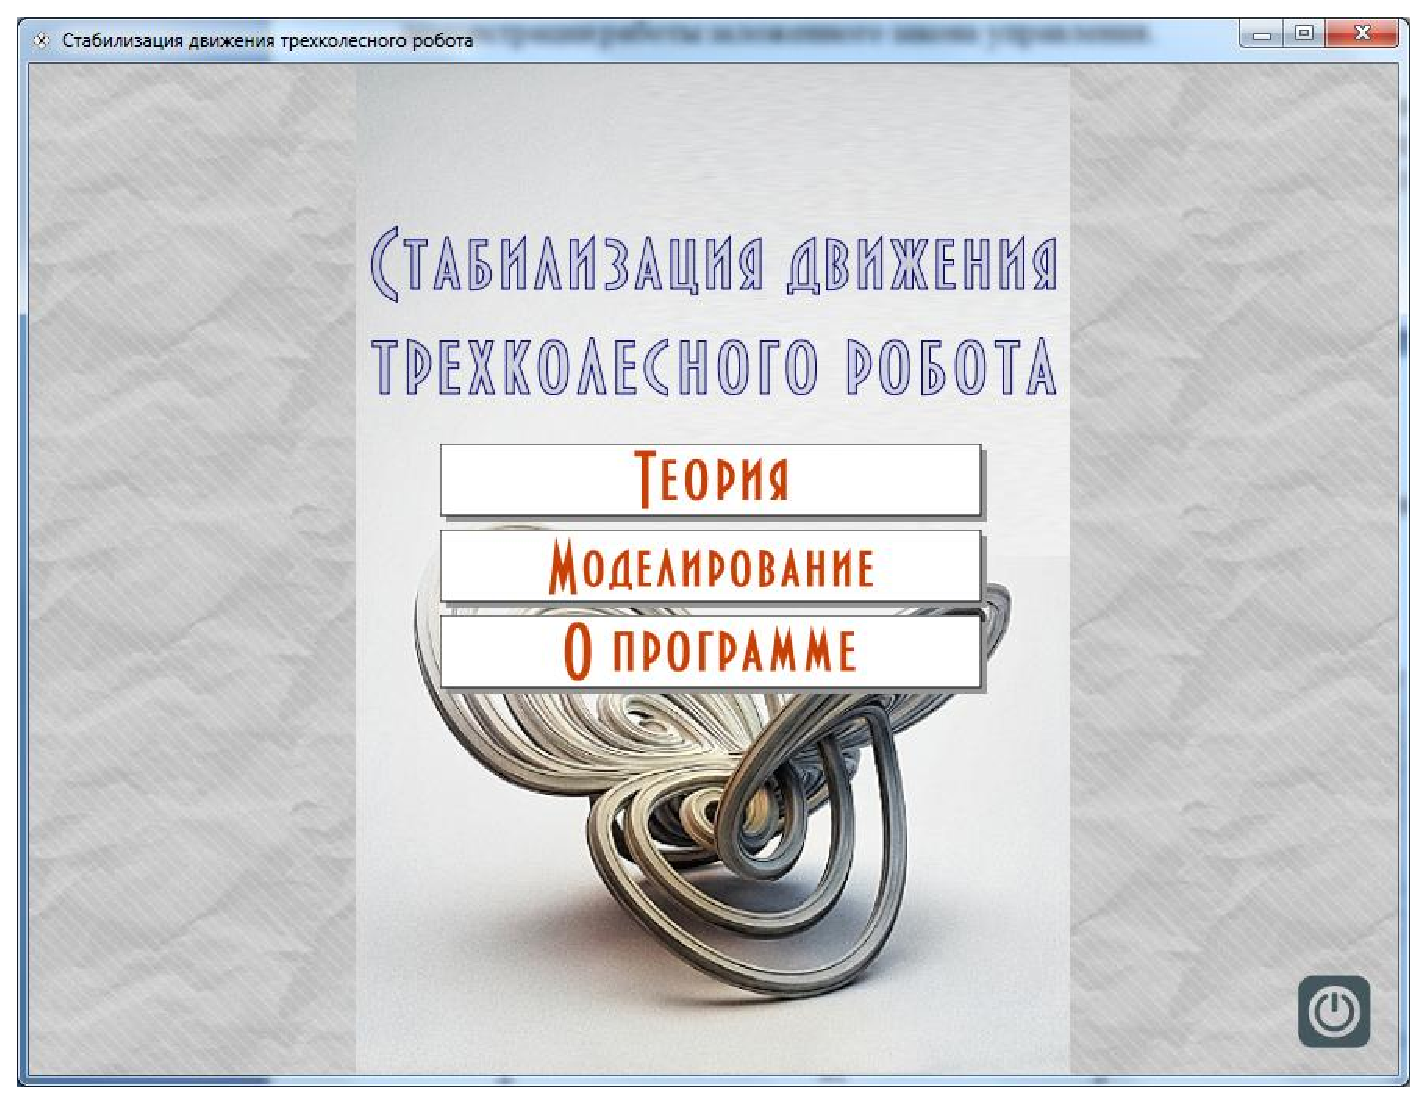
\includegraphics[width=1\linewidth]{window}}
\caption{Основной экран программы}
\label{ris:window}
\end{figure}

\par
\textbf{Теоретический раздел}

В теоретическом разделе содержится схематическое изображение манипулятора, система дифференциальных уравнений, описывающих его движение и краткое теоритеское основание построения управления манипулятором. Подробные теоретические выкладки содержатся в главе 3 настоящей  диссертации.
\nopagebreak[4]
\begin{figure}[h]
\center{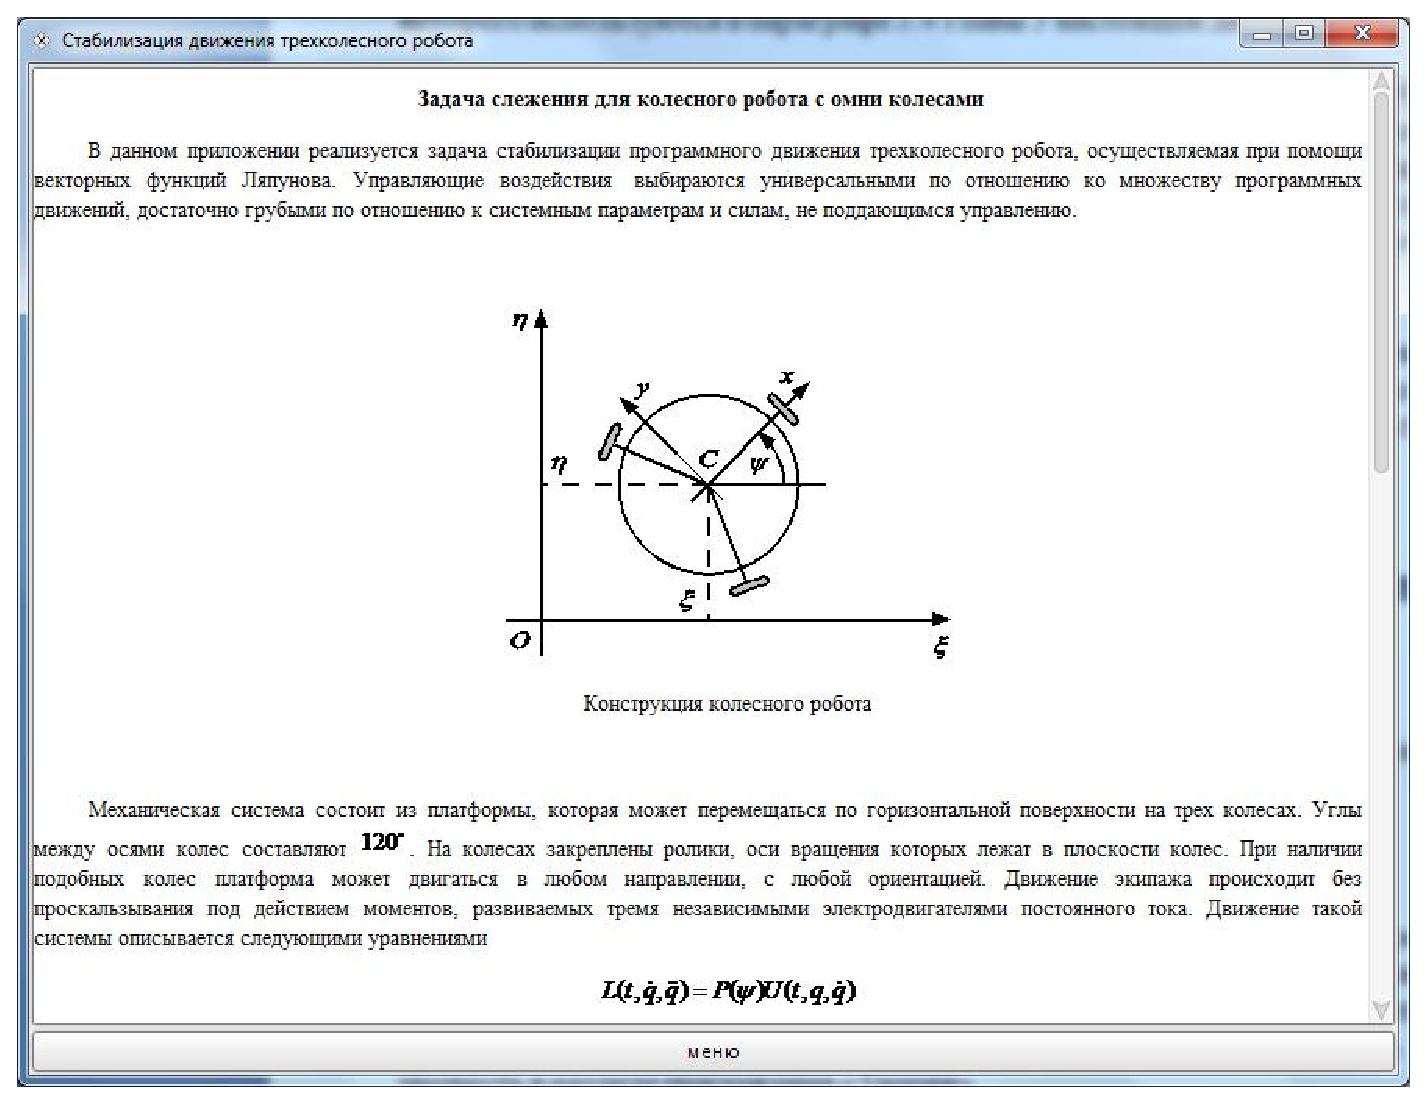
\includegraphics[width=1\linewidth]{theory}}
\caption{Внешний вид теоретического раздела}
\label{ris:theory}
\end{figure} 

\par
\textbf{Раздел моделирование}

В разделе непосредственного моделирования пользователю предлагается задать параметры системы, такие как геометрические характеристики манипулятора (длины звеньев, расстояния до их центров масс), массы звеньев, начальные положения звеньев, а также законы управления в аналитическом виде. Также присутствует возможность автоматического заполенения заранее подобранными значениями по умолчанию для демонстрации работы программы. Значение каждого параметра представлено в теоретическом разделе, на экране моделирования же присутсвуют только сокращенные обозначения, совпадающие с обозначениями в теоретической части.

\begin{figure}[h]
\center{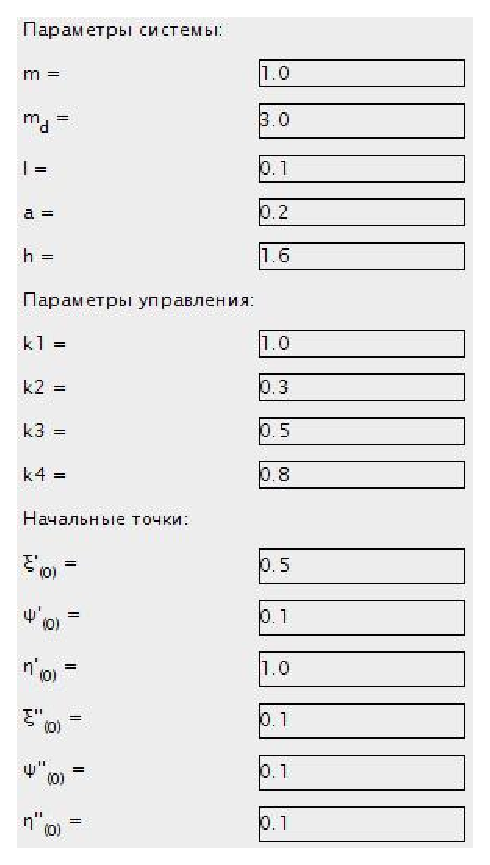
\includegraphics[width=0.5\linewidth]{params}}
\caption{Параметры для расчетов}
\label{ris:params}
\end{figure} 

\begin{figure}[h]
\center{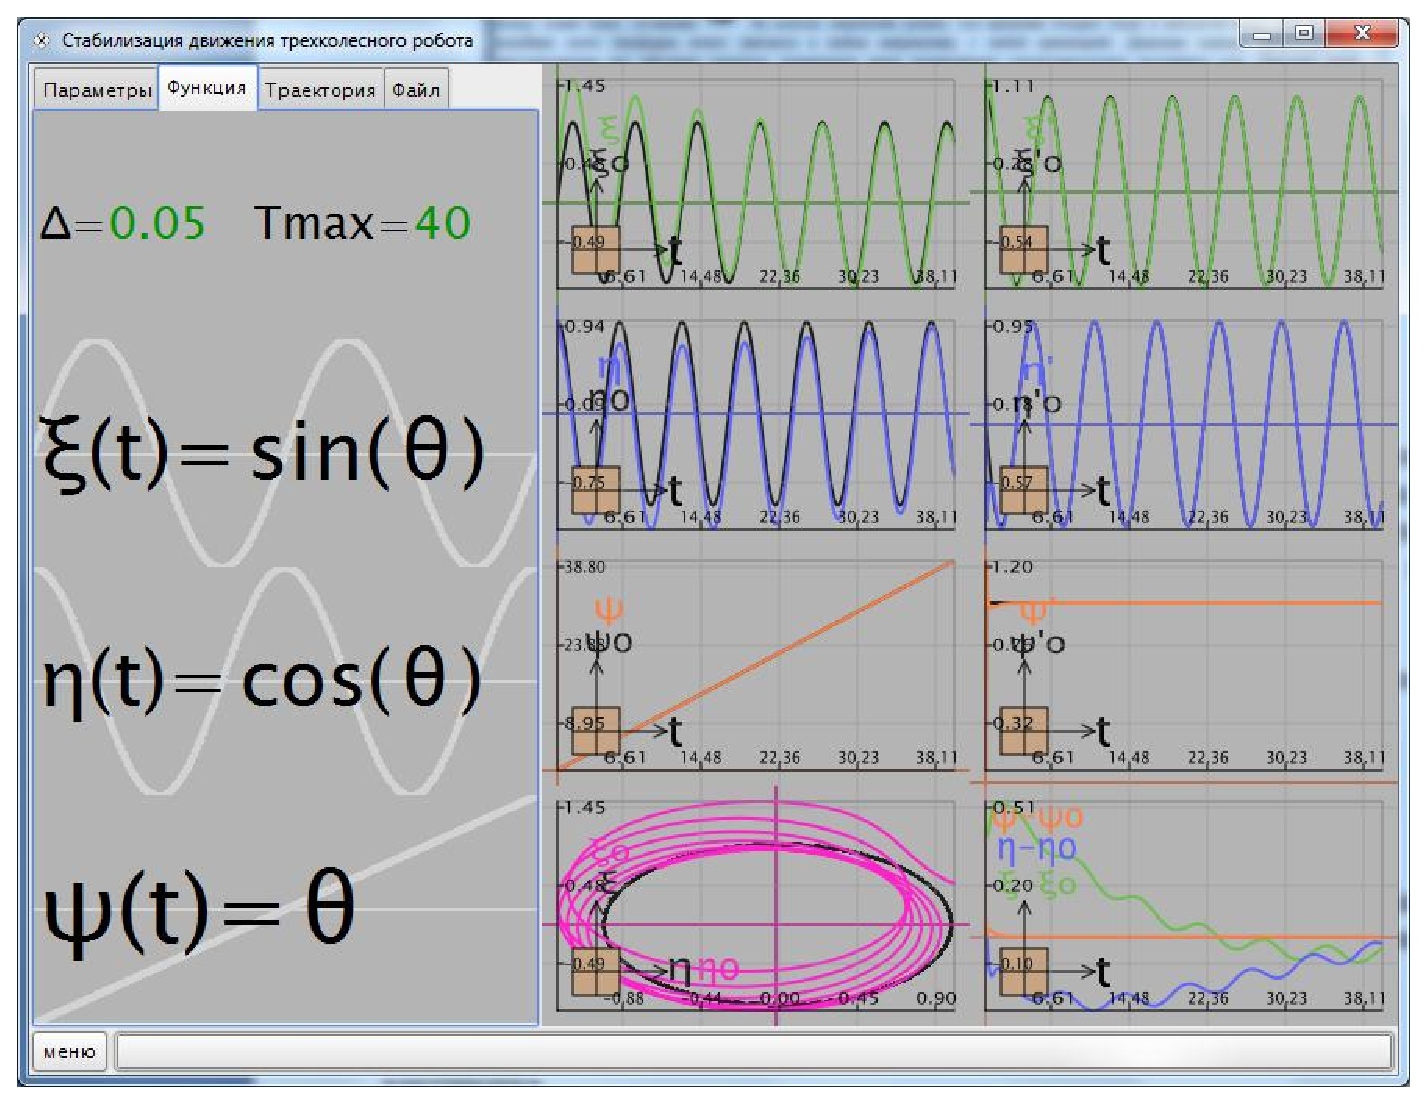
\includegraphics[width=1\linewidth]{modeling}}
\caption{Внешний вид раздела моделирование}
\label{ris:modeling}
\end{figure}

В случае возникновения ошибки, программа сообщает о ней, выделяет незаполненные поля в случае недостаточных данных.
\par
\textbf{Задание закона управления манипулятором аналитически}

Для обработки введенных формул используется открытая сторонняя библиотека, позволяющая пользователю вводить элементарные функции. Также библиотека была доработана для того, чтобы иметь возможность распознавать определенные интегралы с переменным верхним или нижним пределом.

Формулы вводятся в поля ввода в качестве строк текста. В формулах допускается использование констант, основных математических операций и параметров системы, таких, например, как массы звеньев, заданные в виде переменных. При обработке формул происходит преобразование текста в объекты языка Java и сохранение в оперативной памяти. Дальнейшие вычисления проводятся с помощью подстановки вместо переменых констант, необходимых для работы на текущем шаге. Таким образом, обработка формулы производится только на первых шагах, что положительно сказывается на скорости работы программы.

При необходимости библиотке работы с формулами может быть расширена.

Первоначально пользователю предлагается дискретизации $\delta$  и время моделирования  $T_{max}$ рис.\eqref{ris:formul}. После ввода ввода уравнений управления и параметров системы пользователь нажимает на кнопку построения графиков, после чего программа производит моделирование движения манипулятора и отображает результаты в виде графиков, показывающих соответствующее изменение координат каждого из звеньев, а также изменения скоростей звеньев с течением времени, ограничиваясь максимальным временем, заданным пользователем.

\begin{figure}[h]
\center{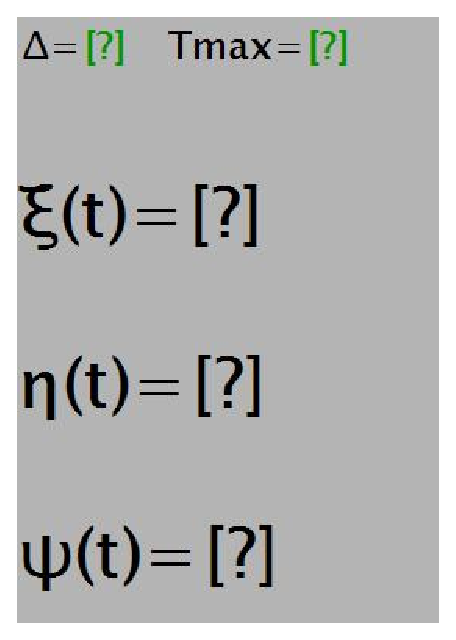
\includegraphics[width=0.5\linewidth]{formul}}
\caption{Система ожидает ввода управления с помощью формул}
\label{ris:formul}
\end{figure}

При наборе формулы поддерживаются следующие действия:
\begin{itemize}
\item{основные математические операции (сложение, вычитание, умножения, деление, возведение в степень);}
\item{ввод формул без ограничения на длину;}
\item{ввод без ограничений по количеству вложенных скобок;}
\item{добавление делегированных тригонометрических и алгебраических функций ($sin(t), cos(t), tg(t), ctg(t), exp(t), ln(t)$ );}
\item{ввод определенных интегралов в том числе с подынтегральной функцией и пределов интегрирования в зависимости от времени $t$;}
\item{ввод независимой переменной $t$;}
\end{itemize}

\textbf{Ввод данных из файла}

При этом вводе данных пользователю необходимо выбрать файл, содержащий заданное управление и параметры системы. В данный момент программой поддерживается два формата хранения данных

\begin{itemize}
\item{cvs;}
\item{json}
\end{itemize}

\begin{figure}[h]
\center{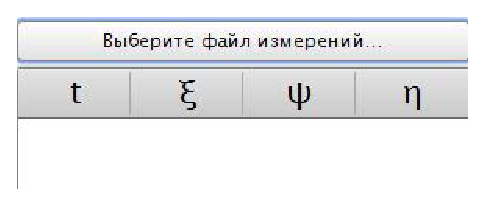
\includegraphics[width=0.5\linewidth]{mass}}
\caption{Внешний вид формы для ввода массива данных}
\label{ris:mass}
\end{figure}

Очередность параметров, считываемых из файла соответсвует порядку их расположения на графическом интерфейсы работы с программой. Так сначала идут параметры системы, затем начальные координаты и скорости звеньев, затем законы управления движением звеньев.

В качества разделителя данных используется символ ";". Дробные числа записываются через символ ".".

\par
\textbf{Расчетная часть}

Для детального ознакомления с реализацией расчета см. Приложение 1.
После задания траектории движения робота одним из описанных способов, в правой части приложения выводятся следующие графики рис.\eqref{ris:graph}

\begin{enumerate}
\item{ графики  $\xi(t), \xi_0(t)$ траектории центра масс платформы }
\item{ графики  $\eta(t), \eta_0(t)$ координаты  центра масс платформы }
\item{ графики  $\psi(t), \psi_0(t)$ угла поворота платформы  }
\item{ графики  $\dot{\xi(t)}, \dot{\xi_0(t)}$ скорости центра масс платформы }
\item{ графики  $\dot{\eta(t)}, \dot{\eta_0(t)}$ скорости координаты  центра масс платформы }
\item{ графики  $\dot{\psi(t)}, \dot{\psi_0(t)}$ скорости поворота платформы  }
\item{ графики траектории платформы  на фазовой плоскости $\xi(\eta(t)), \xi_0(\eta_0(t))$}
\item{ графики  $\|\dot{\xi(t)} - \dot{\xi_0(t)}\|$, $\|\dot{\eta(t)} - \dot{\eta_0(t})\|$, 
$\|\dot{\psi(t)} - \dot{\psi_0(t)}\|$  }
\end{enumerate}
При построении графиков  использовался пятиточечный метод численного дифференцирования.

По графикам можно судить, что рассматриваемая система двигается вдоль отслеживаемой траектории на расстоянии, не превышающем погрешности слежения.

\begin{figure}[h]
\center{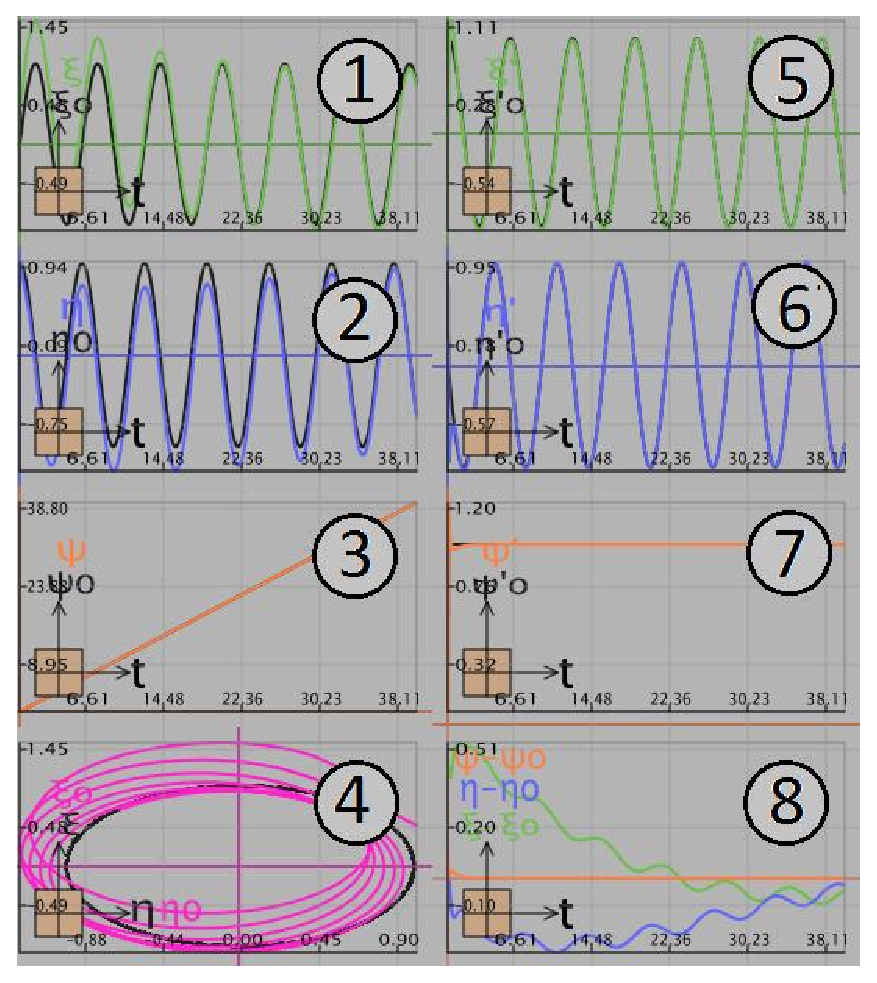
\includegraphics[width=1\linewidth]{graph}}
\caption{Внешний вид расчетной части}
\label{ris:graph}
\end{figure}



\end{document}